\chapter{Extra-tropical cyclones}

% **************************** Define Graphics Path **************************
%\ifpdf
%    \graphicspath{{Chapter3/Figs/Raster/}{Chapter3/Figs/PDF/}{Chapter3/Figs/}}
%\else
%    \graphicspath{{Chapter3/Figs/Vector/}{Chapter3/Figs/}}
%\fi

%
%\section{Characteristics of extra-tropical cyclones}
Extra-tropical cyclones are a dominant feature of the mid-latitudes, associated with strong winds, precipitation and temperature changes. An extra-tropical cyclone is a low pressure system that primarily gets its energy from a horizontal temperature gradient. They have frontal features, i.e. they are associated with cold fronts, warm fronts, and occluded fronts and in the northern hemisphere have winds counter clockwise. Like tropical cyclones, they transport heat and moisture from the Tropics towards the poles and they are embedded in mid-latitude westerlies, travelling in an eastward direction.

%what kind of intensities? named?

\section {Introduction}
\subsection {Formation and structure of extra-tropical cyclones}
%Formation of jet streams? - no, not jet streams
%
%\begin{figure}[h]
%	\centering
%	\noindent\includegraphics[width=20pc,angle=0]{H:/Documents/Admin/ESA/jetstream3.jpg}
%	\caption{North hemisphere cross section showing jet streams and tropopause elevations. Source: \cite{noaa_jetstream}}\label{fig:jetstream}
%\end{figure}

The first conceptualised model of the typical life-cycle of mid-latitude cyclones is the Norwegian model (e.g. Bjerknes and Solberg). This was proposed in the 1910s and 1920s and describes the evolution of a cyclone from an incipient frontal wave with cold and warm fronts, through intensification, maturity and decay (figure \ref {fig:norwegian_maps}).

\begin{figure} % remove [h] and this appeared in the correct place
	\subfloat[Initial state]{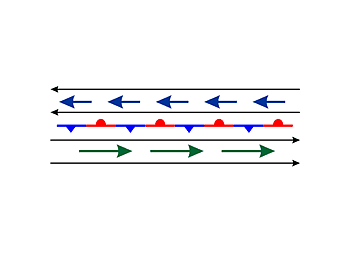
\includegraphics[width=2.0in]{H:/Documents/Admin/ESA/Figures/cyclo1.png}} 
	\subfloat{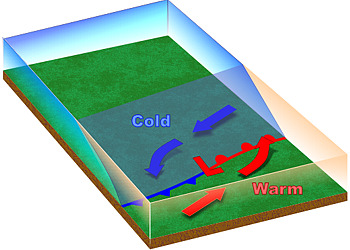
\includegraphics[width=2.0in]{H:/Documents/Admin/ESA/Figures/wave23d.jpg}} 
	\subfloat[Beginning stage]{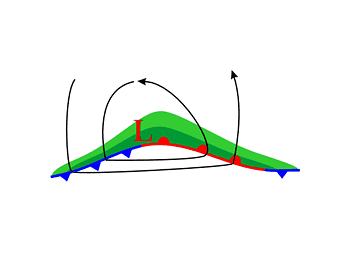
\includegraphics[width=2.0in]{H:/Documents/Admin/ESA/Figures/cyclo2.png}} 
	\subfloat{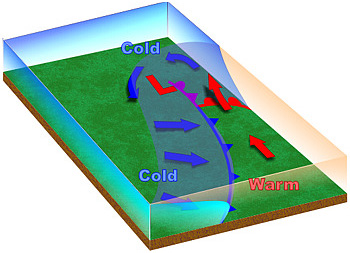
\includegraphics[width=2.0in]{H:/Documents/Admin/ESA/Figures/wave43d.jpg}}  		
	\subfloat[Intensification]{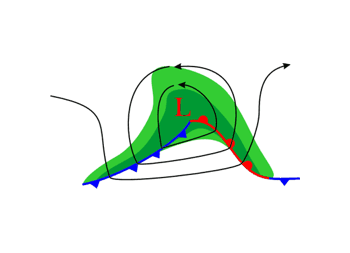
\includegraphics[width=2.0in]{H:/Documents/Admin/ESA/Figures/cyclo3.png}} 
	\subfloat{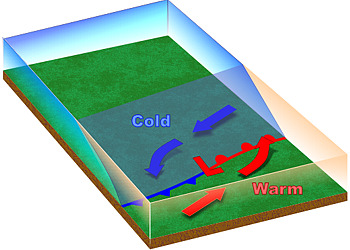
\includegraphics[width=2.0in]{H:/Documents/Admin/ESA/Figures/wave23d.jpg}} 
	\subfloat[Mature stage]{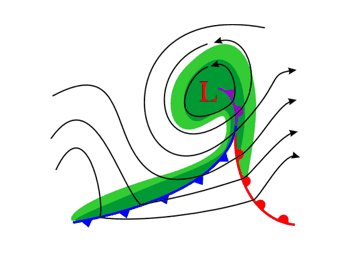
\includegraphics[width=2.0in]{H:/Documents/Admin/ESA/Figures/cyclo4.png}} 
	\subfloat{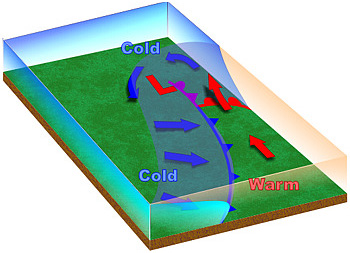
\includegraphics[width=2.0in]{H:/Documents/Admin/ESA/Figures/wave43d.jpg}} 
	\subfloat[Dissipation]{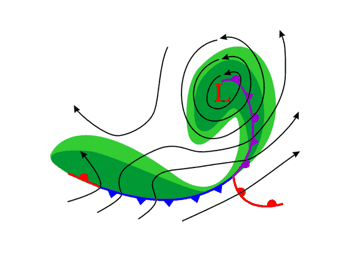
\includegraphics[width=2.0in]{H:/Documents/Admin/ESA/Figures/cyclo5.png}} 
	\subfloat[]{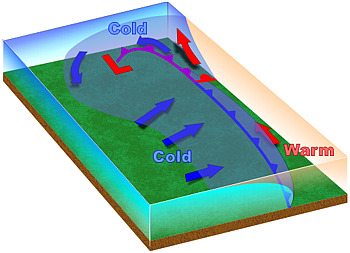
\includegraphics[width=2.0in]{H:/Documents/Admin/ESA/Figures/wave53d.jpg}} 
	
	\caption{The Norwegian cyclone model in (1) map view (2) and 3-D view.  Source: \cite{norwegian}}\label{fig:norwegian_maps}
\end{figure}

One condition that favours cyclogenesis is a baroclinic zone, i.e. a region of large temperature change across a short horizontal distance near the surface, e.g. frontal zones. Above (near the tropopause) and parallel to this baroclinic zone is often a strong jet stream, driven by the thermal wind effect \ref{stull}. A wave develops on the front as an upper level low pressure system embedded in the jet stream moves over the front. As the air masses begin to rotate, defined cold and warm fronts develop. The wave intensifies and the low pressure centre deepens. The warm sector narrows as the cold front rotates around the cyclone faster than the warm front, and an occluded front develops where the cold front overtakes the warm front. As the cold front continues advancing on the warm front, the occlusion increases and eventually cuts off the supply of warm moist air, causing the low pressure system to gradually dissipate \citep{norwegian}. Precipitation occurs as air is forced to rise ahead of the warm front and the cold front. The more dense cold air undercuts the warm air and the less dense warm air rises above the cold air.

%http://weatherfaqs.org.uk/node/98
%As with the Norwegian cyclone model, the Shapiro-Keys model has an incipient cyclone develops cold and warm fronts, but in this case, the cold front moves roughly perpendicular to the warm front such that the fronts never meet, the so-called 'T-bone'. Also, a weakness appears along the poleward portion of the cold front near the low center, the so-called 'frontal fracture' and a back-bent front forms behind the low center. (In the final stage), colder air encircles warmer air near the low center, forming a warm seclusion. 

An alternative model is the Shapiro-Keyser model. The main difference from the Norwegian model is that the cold front moves roughly perpendicular to the warm front and they never meet. The occluded front is due to a weakness in the cold front near the low centre.
%The occluded front is an extension of the warm front rather than a result of the cold front catching up with the warm front. Both are valid and suited to different scenarios.. e.g....

%Conditions favourable to cyclogenesis are a baroclinic atmosphere (a region of large temperature change across a short horizontal distance near the surface), there is often an associated a strong jet stream running parallel at upper levels.
%what about mositure?
%cyclogenesis involves sea-level pressure decrease as the low pressure centre deepens, upward-motion increase, and vorticity increase.

Energy from baroclinicity in the atmosphere. This is in contrast to tropical cyclones, where there is little temperature contrast across them and they get their energy from the underlying ocean. Much like tropical cyclones, extra-tropical cyclones are moved by the jet stream and by other large-scale components of the global circulation \citep{stull}.

%Baroclinic instability is due to a horizontal temperature gradients in a rotating environment. 

%What season? winter storms or summer storms? extratropical transition?

%extratropical ocean-atmosphere interaction dominated by atmosphere forcing the ocean, but with variability with oceanic processes more important to SST in the vicinity of WBCs (smirnow).

%baroclinic wave, steering level. Steered by large scale, much like TCs?

Figure \ref{fig:ET_structure} shows a mature extra-tropical cyclone in more detail. An extra-tropical cyclone is typically larger than an average tropical storm, (approximately 1000 km)
As an extra-tropical cyclone moves eastwards, ahead of the warm front, there stratiform cloud as warm air is forced to rise and cool. Behind the warm front is the warm sector, of relatively warm air and generally clear skies. At the cold front, dense cool air undercuts the warm, moist air and forces it steeply upwards, with a band of cumuliform clouds, heavy rain and thunderstorms. Following the passage of the cold front, there is cooler air, bright skies and showers, and a marked veer in wind direction. The near surface winds converge towards the low pressure centre. Structurally, extra-tropical cyclones are 'cold-core', unlike tropical cyclones, which are 'warm core'.
%Cold sector surface flow is from the northwest
%Warm sector surface flow is from the southwest, bringing warm low-latidude air poleward and upward 'warm conveyor belt', associated with weak turbulent heat fluxes at the surface (warm path pahper?). Warm conveyor belt, cold conveyor belt, dry intrusion.

\begin{figure}[h]
	\centering
	\noindent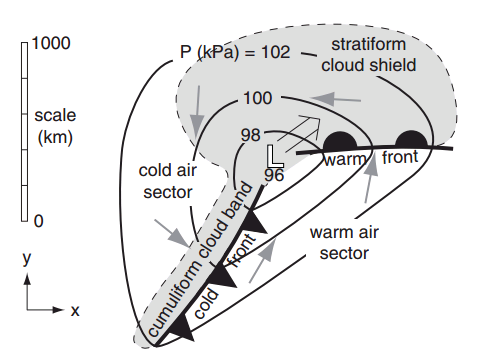
\includegraphics[width=20pc,angle=0]{H:/Documents/Admin/ESA/Figures/ET_structure.png}
	\caption{Components of a typical extra-tropical cyclone in the N. Hemisphere. Light grey shows clouds, dark grey arrows are near-surface winds, thin black lines are isobars (kPa), thick black lines are fronts, and the double-shaft arrow shows movement of the low centre 'L'. Source: \cite{stull} }\label{fig:ET_structure}
\end{figure}


%\section {Impact of extra-tropical storms}

\subsection {Extra-tropical storm activity} %ocean, atmos, variability
%
Much like with tropical cyclones, the variability of extra-tropical storm activity is due to both atmospheric and ocean conditions. These storm systems extend through the atmosphere, however, underlying conditions in the MBL are important too. The marine boundary layer (MBL) is the part of the atmosphere that lies over the ocean surface and is directly influenced by it.  Variations in the ocean surface therefore affect the cyclone, affecting ocean-atmosphere exchanges of heat, moisture and momentum.

%Due to variations in the atmosphere and ocean - baroclinic atmosphere required for cyclogenesis (ref section). 

Extra-tropical storms are driven by strong temperature gradients (section 3.1) and in the North Atlantic, often develop in baroclinic zone over Gulf Stream. In the MABL, the Gulf Stream directly influences air temperature and pressure fields but also has effects throughout the entire troposphere, with upper-tropospheric divergence exhibiting a structure similar to the surface convergence and precipitation patterns, all meandering with the Gulf Stream (\citep{minobe2008influence}).
%Major storm tracks are organised along or just downstream of the main oceanic frontal zones (Nakamura et al 2004).
%Sheldon(The atmosphere above the Northern Hemisphere’s western boundary currents (the Gulf Stream and Kuroshio) are maximums in the winter atmospheric variability on a synoptic timescale of 2-6 days (Lau and Wallace, 1979; Blackmon, 1976; Hoskins and Valdes, 1990). These regions of synoptic variability are called the storm tracks and the variability is measuring the growth of extra-tropical cyclones that occur there (Dacre and Gray, 2009).)

In the marine atmospheric boundary layer (MABL), the Gulf Stream directly influences air temperature and pressure fields locally and also throughout entire troposphere, with upper-tropospheric divergence exhibiting a structure similar to the surface convergence and precipitation patterns, all meandering with the Gulf Stream (\cite{minobe2008influence}). Extra-tropical storms are driven by strong temperature gradients and in the North Atlantic, often develop in the baroclinic zone over Gulf Stream. Here, strong oceanic fronts that help to maintain the strong baroclinicity that is required to maintain them \citep{nakamura2004observed, nakamura2008importance, hoskins1990existence}

%\cite{nakamura2004observed}
%As the surface air temperature over the open ocean is linked to SST underneath, maritime surface baroclinic zones tend to be anchored along oceanic fontal zones [NS04]. Though acting as thermal damping for the evolution of individual  eddies, heat exchange with the underlying ocean, on longer time scales, can act to restore atmospheric near-surface baroclinicity against the relaxing effect by atmospheric eddy heat transport, as evident in sharp meridional contrasts in upward turbulent heat fluxes observed climatologically across midlatitude frontal zones [Oberhuber, 1988]. Some observations are shown in section 2 to suggest that SST anomalies in a midlatitude frontal zone can likely play a more active role in the air–sea interaction than act to damp  tmospheric anomalies thermally Hoskins and Valdes (1990) mean diabatic heatin as a result of the warm ocean current restores the meridional atmostpheric temperature gradient and therfore baroclinciiy, that is vital to the storm tracks existence.

%nakamura et al 2008 \cite{nakamura2008importance}
%and booth et al 2010 - air-sea heat exchanges at oceanic fronts restore the baroclinicity of the atmosphere at low levels.
%shear instability not parametrised in current generation of GCMs.

%GCMs generally simulate the storm tracks well (d'Andrea et al 1998)as they are large-scale phenomenon of the atmospheric circulation. Also climate models can capture the structure of ETCs (cite{\catto2010can}).
%Atmosphere-ocean interactions are their strongest over WBCs, e.g Gulf Stream. Strong fluxes of heat and moisture anchor the storm tracks to the WBCs (Nakamura et al 2004). allows for recurrent develpoment of storm tracks - creates baroclinicity?

%Deep ascent over the Gulf Stream is a result of extreme events, i.e. extra-tropical storms \citep{minobe2008influence}(check this)
%The storms occur in these locations as the strong oceanic fronts help maintain the surface baroclinicity required to produce them (Nakamura and Shimpo, 2004 Nakamura et al., 2008; Sampe et al., 2010).  (sheldon thesis).
%SHELDON THESIS:
%The Gulf Stream is the western boundary current for which the most links to deep convection have been found. %The deep ascent over the Gulf Stream found by Minobe et al. (2008) is a result of extreme events that skew the mean to ascent, and their results do not represent an average day in that region. The ascent above the Gulf Stream being a product of extreme events is consistent with the region also being the centre of action for winter synoptic systems in the Northern Hemisphere (Hoskins and Valdes, 1990).


\subsubsection {The Gulf Stream}

Global atmospheric circulation is characterised by easterly trade winds in the Tropics and the westerlies in the mid-latitudes.  The atmosphere exerts a force on the ocean below, which is also affected by the rotation of the earth, a factor which increases with proximity to the poles. Surface currents located on the western side of ocean basins are must faster than on the east and are among the fastest surface currents in the ocean (\citep{nasa_ocean}).  These currents also extend much deeper than most other surface currents, and are deflected by the continental margins, which prevent these currents from flowing onto the shallow continental shelves \citep{nasa_wbc}.
%Waters in western boundary currents (WBCs) typically move 40 to 120 km (25 and 75 mi) per day (\citep{nasa_wbc}). 
The Coriolis effect increases with latitude, and so is stronger in the latitudes of the westerlies than in the latitudes of the equatorial trade winds. Surface waters build up on the western side of ocean basins, resulting in the ocean-surface slope to be steeper on the western side (versus eastern side), which leads to a faster geostrophic flow on that side \citep{nasa_wbc}.

The Gulf Stream can be seen in Sea Surface Temperature data (SST), transporting a warm tongue of water poleward and eastward (figure \ref{fig:GS_map}). On the northern edge, there is a strong SST gradient while to the south, eddies tend to erode this gradient.

\begin{figure}[h]
	\centering
	\noindent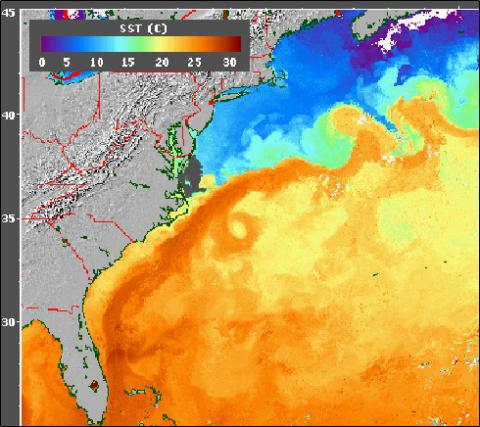
\includegraphics[width=14pc,angle=0]{H:/Documents/Admin/ESA/Figures/GulfStream.jpg}\\
	\caption{The Gulf Stream, revealed through SST data, made from the AVHRR (Advanced Very High Resolution Radiometer) sensor carried on a NOAA satellite. In this image, purple and blue represent the coldest temperatures (between 0-15 $^0$C) and orange and red represents the warmest temperatures (between 22-32 $^0$C). Source: \cite{gsnasa}}\label{fig:GS_map}
\end{figure}


%Deep ascent over the Gulf Stream is a result of extreme events, i.e. extra-tropical storms \citep{minobe2008influence}(check this)

It has been found that these extra-tropical storms occur in locations such as the Gulf Stream, where there are strong oceanic fronts that help to maintain the strong baroclinicity that is required to maintain them (Nakamura and Shimpo, 2004 Nakamura et al., 2008).
%The storms occur in these locations as the strong oceanic fronts help maintain the surface baroclinicity required to produce them (Nakamura and Shimpo, 2004 Nakamura et al., 2008; Sampe et al., 2010).  (sheldon thesis).

%heat from the tropics poleward - affects cyclogenesis (how is this related to temp?)


\subsection{The warm path}

Previous studies \cite{vanniere2017cold} \cite{sheldon2017warm} have suggested a new mechanism by which the SST distribution of the Gulf Stream impacts cyclones over the North Atlantic Ocean. The mechanism consists in an intensification, and possibly a destabilization, of the frontal circulation embedded in the cyclones. 

The 'warm path' is the mechanism of oceanic forcing  associated with impact of the Gulf Stream warm tongue on the warm sector of cyclones. Here there are weak air-sea heat fluxes, which is in sharp contrast to what occurs in their cold sector.

In \cite{sheldon2017warm} , this warm path mechanism has been examined using one case study on January 14th 2004, with a MetUM simulation (12km) integrated for 72 hours. A 'SMTH' experiment used a smoothed Gulf Stream warm tongue SST, a 'COOL' reduced the SST everywhere by 3K and the control used an unperturbed SST. Results showed that the Gulf Stream has a significant impact on the upward motion present in the cyclone, with back trajectories providing a useful tool. 

\begin{figure}

	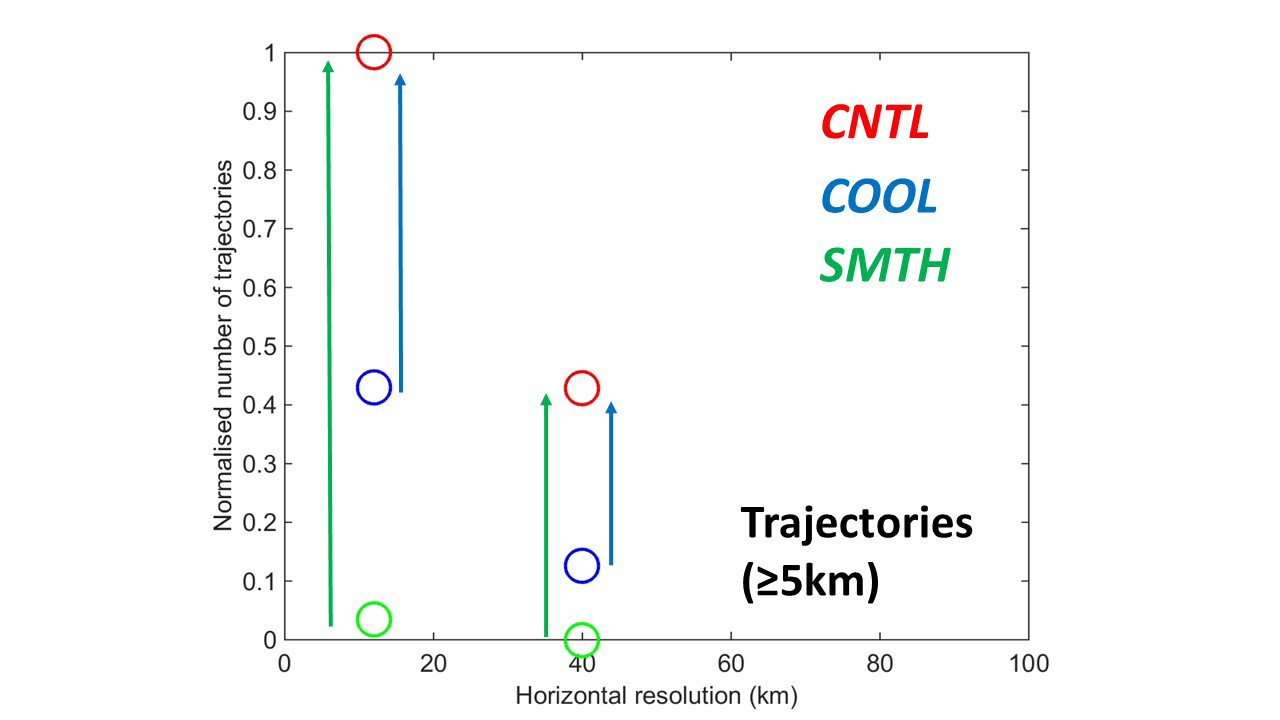
\includegraphics[width=22pc,angle=0]{H:/Documents/Admin/ESA/Figures/warmpath_result.png}
	\caption{Number of back trajectories (circles) with heights z 5km at t=24h and reaching low levels over the ocean at t=0h: red for CNTL, blue for COOL and green for SMTH. The arrows indicate a measure of oceanic forcing when comparing CNTL,SMTH or CNTL,COOL. Normalized such that the number for CNTL at 12km resolution is unity. Source: Sheldon et al. 2016}\label{fig:wp_result}
	\centering
\end{figure}

Figure \ref{fig:wp_result} shows that at both model resolutions (12 km and 40 km), the control simulation has more than double the number of trajectories that the perturbed simulations, with the smooth simulation having a the fewest. Oceanic forcing is measured by the number of trajectories as this is related to upward mass transport, which scales with the diabatic heating (due to condensation of water vapour carried in the flow) in the ascending branch (Sheldon et al., 2016).

Thermodynamic and dynamic mechanisms have been proposed. For the thermodynamical mechanism, in the control experiment trajectories are parallel to the Gulf Stream, with no significant loss of heat and possible gain of moisture, maintaining high $\theta$e values. In the smooth simulation, air parcels cross SST contours, reducing $\theta$e and the likelihood of ascent. The dynamical considerations are that, due to stronger SST gradients in the control experiment, a thermally driven cell enhances the frontal circulation, increasing the feed into the warm conveyor belt. Also, it is possible that the stronger SST gradients destablise the frontal circulation by enhancing the vertical wind shear (Sheldon et al., 2016).

%Partitioning between bottom or top heavy feeding of the ascent from low levels is primarily set by SST gradient. Ability for air parcels to ascent in the WCB sensitive to the absolute SST.

%Dynamical diagnostic in ERA-Interim, suggests Gulf Stream warm tongue should have most frequency vigorous ascent from low levels in the NW Atlantic in winter.
%Climatological distribution of WCBs in the NH winter peaks over the Gulf Stream warm tongue.

This study \cite{sheldon2017warm}  focussed on one case study, and it will be valuable to explore this mechanism in more cases. Also just one model realisation, so examine other models (ref chapter) and other cases (ref chapter).


%Climate models (HiGEM (0.83x1.25) and ERA-40) can capture the structural features of extra-tropical cyclones \citep{catto2010can} analysing warm conveyor belt, cold conveyor belt and dry intrusion.

Explain in depth PV and equivalent potential temperature\\


\subsection{Atmospheric instability and convection}

\subsubsection {Gravitational instability and upright convection}

In a hydrostatically balanced atmosphere, the mean-state potential temperature ($\theta$) decreases with height. If the potential temperature cools with height, there will be overturning as the cool air sinks. This is gravitational instability (\ref{eqgravinst}), which releases upright convection and is purely vertical.

\begin{equation} \label{eqgravinst}
\frac{d\theta}{dz} < 0
\end{equation}


\subsubsection {Inertial instability and horizontal movement}
Inertial instability operates in the horizontal plane and is detected by absolute momentum (M). Absolute momentum, as defined by \cite{eliassen1962vertical} is the rotation of the Earth plus the rotation due to variations in the wind field:

\begin{equation} \label{eqM}
M = V + fx
\end{equation}


%\begin{equation} \label{eqN}
%N = U - fy
%\end{equation}

where V is the frontal velocity and x is the distance along the transverse plane to the front. When the absolute momentum decreases in the x-direction then the atmosphere is unstable:

\begin{equation} \label{eq_iner_inst}
\frac{dM}{dx} < 0
\end{equation}


\subsubsection {Shear (symmetric) instability and slantwise convection}

Shear (or symmetric) instability is a combination of gravitational and inertial instability. A parcel may be inertially stable to horizontal displacements and gravitationally stable to vertical displacements, but may be unstable to slantwise displacements by shear instability. 

A barotropic atmosphere is one where the density depends solely on pressure, whereas in a baroclinic atmosphere the density depends on both the temperature and the pressure. In a barotropic flow, potential temperature surfaces (isentropes) are horizontal and absolute momentum surfaces (M) are vertical. In a baroclinic environment, the isentropes tilt upwards on the cold side and downwards on the warm side. The absolute momentum surfaces slope in response to the vertical shear from thermal wind balance, tilting up on the cold side and down on the warm side.
%
%\begin{figure}[h]	
%	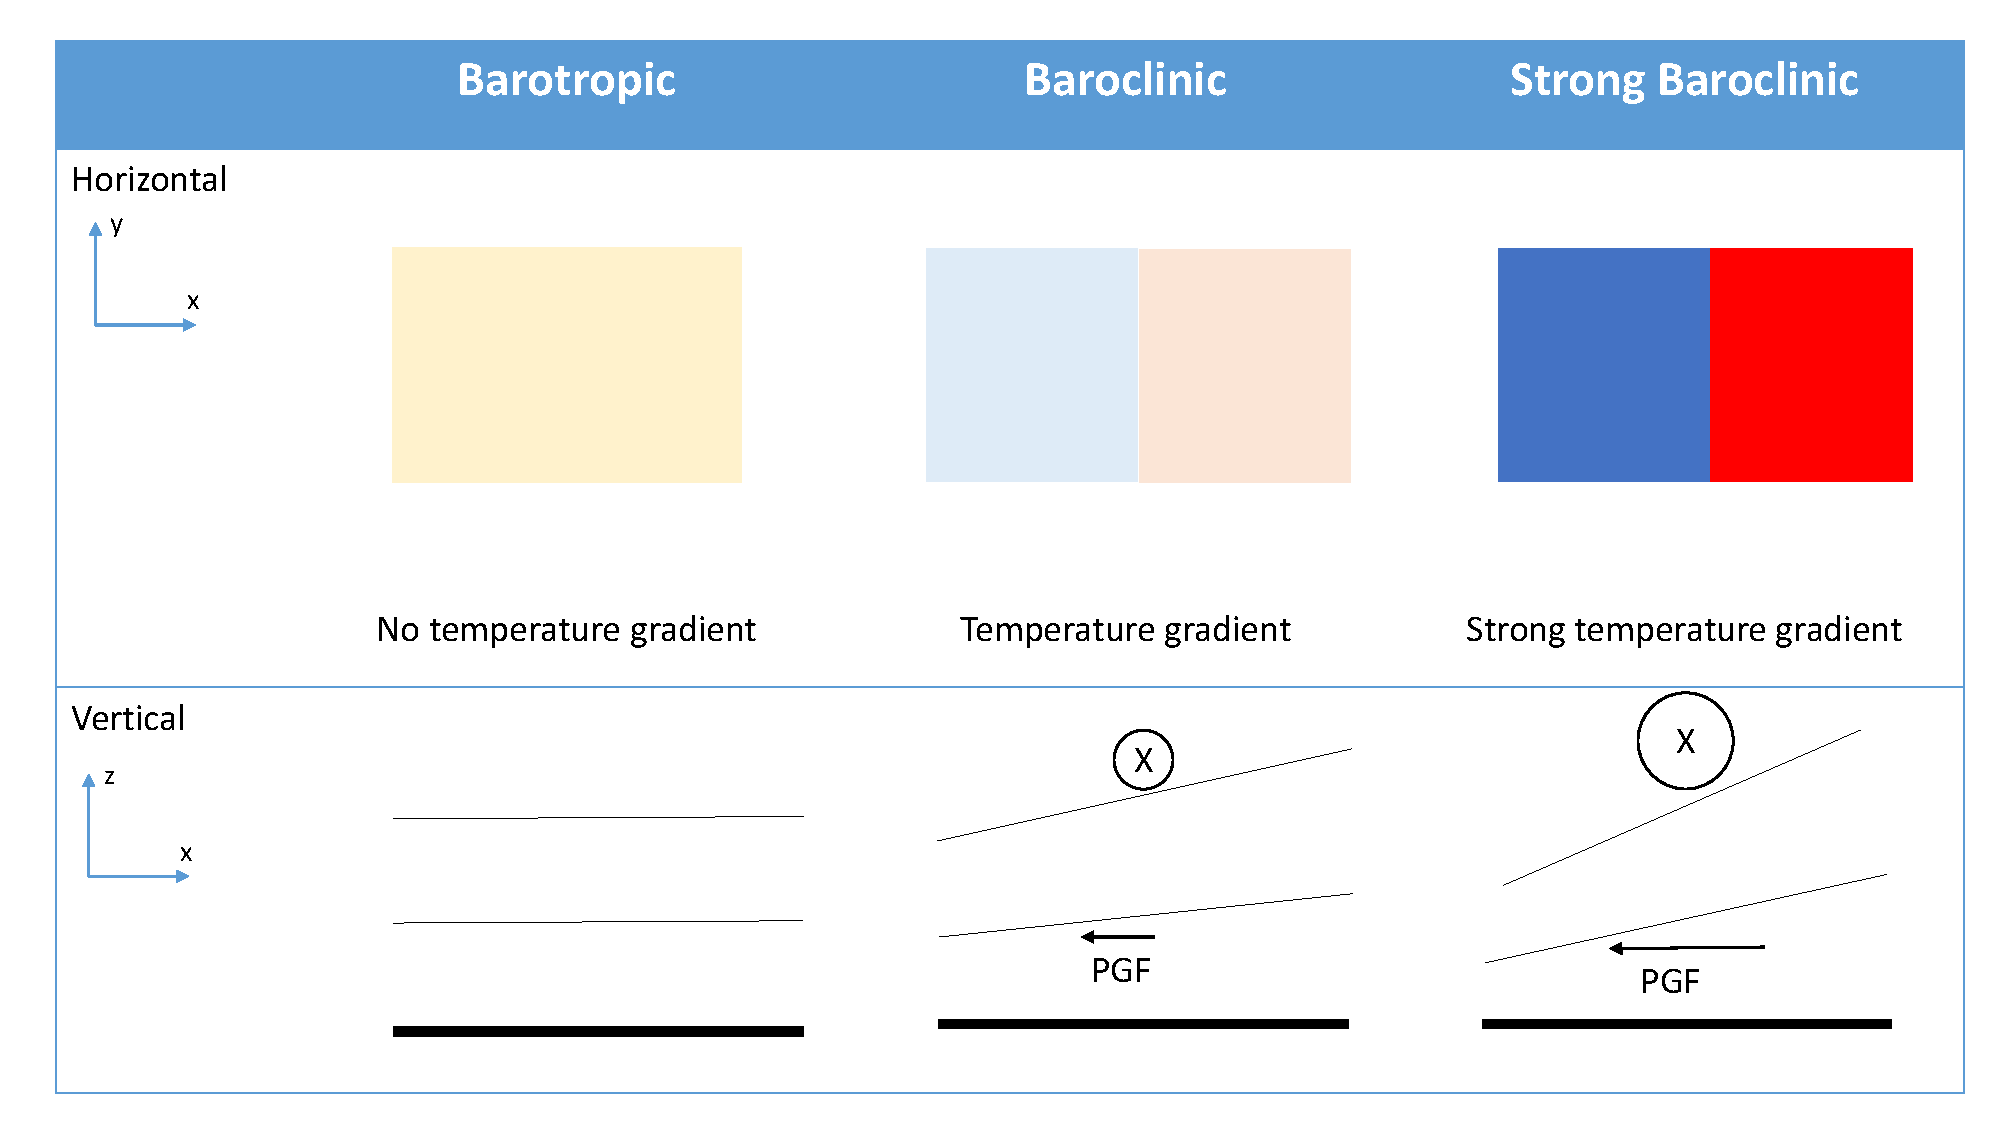
\includegraphics[width=34pc,angle=0]{H:/Documents/Thesis/phd-thesis-template-2.2.2_AC/phd-thesis-template-2.2.2/Figs/barotropic2_new.pdf}
%	\caption{Barotropic and baroclinic environments in the horizontal and vertical, and resultant pressure gradient force (PGF) and thermal wind (cross in circle). Thin black lines are isentropes.}\label{fig:barotropic}
%	\centering
%\end{figure} 

The  M-$\theta$e relationship states that if the $\theta$e surfaces are steeper than the M surfaces, there is symmetric instability. Any slantwise displacement occurring between the slopes of these surfaces will release the symmetric instability and the parcel will be accelerate in the direction away from the original position. Figure \ref{fig:symm_inst} illustrates the M-$\theta$e relationship, with a symmetrically unstable atmosphere on the left and a symmetrically stable atmosphere on the right. Only moist slantwise instability occurs in the Earth's atmosphere \cite{bennetts1979conditional} and so $\theta$e is used. This instability has a 2D assumption that there is no variation in the along front direction. 


\begin{figure}
	\centering	
	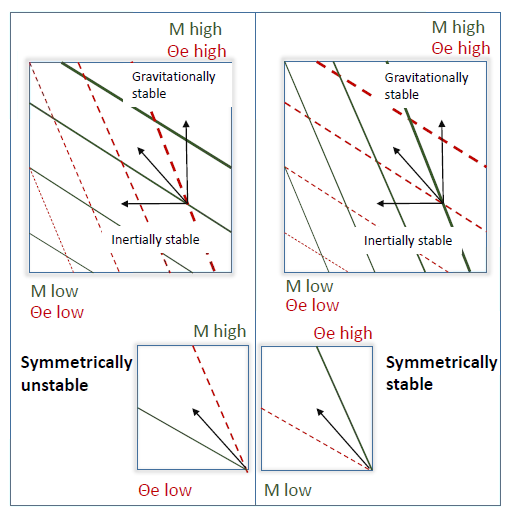
\includegraphics[width=26pc,angle=0]{H:/Documents/Thesis/phd-thesis-template-2.2.2_AC/phd-thesis-template-2.2.2/Figs/mocrette_diagram2_screen.png}
	\caption{Shear (symmetric instability). Isentropes are shown in red dashed lines and lines of constant absolute momentum (M) in solid green. Thickness of the lines increases towards  higher values. Both environments are baroclinic and $\theta$e and M are low in the bottom left and high in the top right. The black arrows show direction of movement of air parcels. In both panels a and b, if a parcel is moved to the left, it is inertially stable as it is moving towards an area of reduced absolute momentum. In both panels a and b, if a parcel is moved vertically, they are gravitationally stable as potential temperature is increasing in this direction and so the parcel will return to it's original position. However, in panel a, if an air parcel is moved along arrow x, it is moving towards lower potential temperature and high M, so is symmetrically unstable. In panel b, it will move towards higher $\theta$e and low M, and is symmetrically stable. Modified from \cite{morcrette2004radar}}\label{fig:symm_inst}
\end{figure}


%\begin{figure}
%	\centering	
%	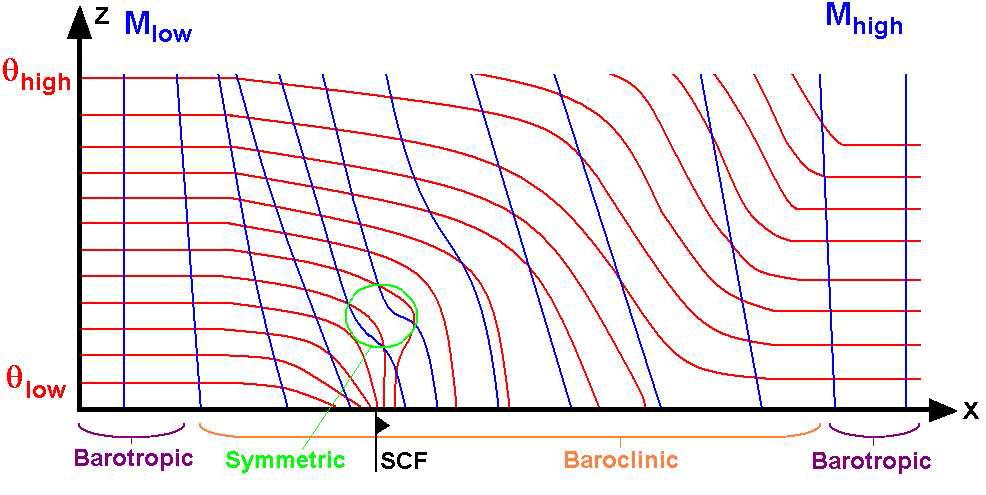
\includegraphics[width=26pc,angle=0]{H:/Documents/Thesis/phd-thesis-template-2.2.2_AC/phd-thesis-template-2.2.2/Figs/morcrette_cx.png}
%	\caption{1.6 The distribution of saturated equivalent potential temperature (red lines) and
%		geostrophic absolute momentum Mg (blue lines) in the broad region around a cold front. Far
%		from the front, the atmosphere is barotropic, within the cold frontal region the atmosphere is
%		increasingly baroclinic, very close to the front, a conditionally symmetrically unstable region
%		may be present. In this example, there is also a small region of conditional instability below
%		the symmetrically unstable region.Source: \cite{morcrette2004radar}}\label{fig:symm_inst2}
%	
%\end{figure}

It has been suggested that slantwise convection from the release of shear instability can explain banded precipitation often seen at cold fronts \citep{bennetts1979conditional, seltzer1985possible}, caused by cells of alternating rotation creating updrafts and downdrafts.

The shear instability diagnostic that is used in this study is diagnosed using:
% dubar/dp x (u'w')bar + dvbar/d[ x (v'w')bar
\begin{equation} \label{eq_diag}
-\overline{w'u'} . \frac{\partial{\overline u}}{\partial z} + \overline{w'v'} . \frac{\partial{\overline v}}{\partial z}
\end{equation}

\begin{equation} \label{eq_diag}
\frac{\partial}{\partial{T}} EKE = -\overline{w'u'} . \frac{\partial{\overline u}}{\partial z} + \overline{w'v'} . \frac{\partial{\overline v}}{\partial z} + ...
\end{equation}

The instability in the x (u) and y (v) directions are combined. The covariance of small-scale vertical motions ($\omega$') and horizontal vertical motions (u' or v') is calculated and then the  product with the vertical shear of low pass winds ($\overline{u}$ or $\overline{v}$)  is created. This is a momentum flux that is purely mechanical and has no dependence on temperature.

%Energy cascade. Also small scale feeds back on the large scale - the diagnostic is the bar value.
%
%Mechanical only.... not like capes????
%Thermodynamic and dynamic mechanism???? what is all this about?
%Shear diagnostic is just vertical and horizontal winds.

%Holton P 279 - symmetric baroclinic instability
%Absolute momentum and potential temperature conservation
%
%WHAT IS MOMENTUM AND ENERGY
%
%\begin{equation} \label{eq_EKE}
%\frac{\overline{(u'^{2}+v'^{2})}}{2} 
%\end{equation}
%EKE in relation to diagnostic?


%Buoyancy (b). g is acceleration due to gravity \(9.8ms^{-1}\). {$\rho$} is density.
%
%\begin{equation} \label{eq_b}
%b = -g\frac{\rho}{\rho_0}
%\end{equation}
%
%Also calculated upright buoyancy (w'{$\alpha$})
%
%Relate to buoyancy and EKE




\subsection{Observations of extra-tropical storms}


\subsection {Representation in models}

%Different results - different identification and tracking, intensity measures \citep{ulbrich2009extra}.

%Climate models (HiGEM (0.83x1.25) and ERA-40) can capture the structural features of extra-tropical cyclones \citep{catto2010can} analysing warm conveyor belt, cold conveyor belt and dry intrusion.

\section {Research question..}
Extra-tropical cyclone activity in the North Atlantic and the relationship with the sea surface temperature in the Gulf Stream region. I will assess whether or not the warm path mechanism (Section 3.3), already examined in one case study \cite{sheldon2017warm}, has relevance to the climatological state of the storm-track in the North Atlantic. I will analyse operational and ensemble forecasts run at ECMWF (1980 to present at a resolution of 9km and 16km, respectively) using diagnostics to isolate the new mechanism that have already been developed. These show the presence of regions of negative PV at mid to upper levels, downgradient vertical momentum fluxes by small spatial scales. The new work proposed here will complement my first years work of statistical analysis with a more physics-based and model-based approach. It will also offer a broader view of how the ocean state affects cyclones worldwide. 

ADD TO ACRONYMS: HRES, AGCM, OGCM.

% from lecturev3 latex doc - looks wrong
%\frac{dQ}{dt} & =0\\
%Q & \equiv\frac{\zeta+f}{H+\eta}


\section {Data}  \label{data}

The data used analysed has been produced by ECMWF. The ERA-Interim reanalysis (ref) and acknowledge and the ECMWF forecast hindcast and forecast, which are described in detail along with the model in section \ref{ECMWF_fs}.

\subsection {ECMWF Integrated Forecasting System (IFS)}  \label{ECMWF_fs}
%www.ecmwf.int/en/forecasts/documentation-and-support is ecmwf_ifs in jabref
%ecmwf_user_guide
%ecmwf_ifs_dynamics
%ecmwf_atm_dyn
%ecmwf_newgrid

The ECMWF Integrated Forecasting System (IFS) consists of an atmospheric general circulation model (AGCM), an ocean general circulation model (OGCM, res), an ocean wave model, a land surface model, along with perturbation models for the data assimilation (EDA) and forecast (ENS) ensembles.

"The dynamical core of IFS is hydrostatic, two-time-level, semi-implicit, semi-Lagrangian and applies spectral transforms between grid-point space (where the physical parametrizations and advection are calculated) and spectral space." \citep{ecmwf_atm_dyn}. In the horizontal, a type of reduced Gaussian grid is used (check the new one is reduced Gaussian), where the separation between longitudinal points is kept almost constant with increasing latitude, by gradually decreasing the number of grid points towards the poles. "For the convenience of computing horizontal derivatives and to facilitate the time-stepping scheme, a spectral representation, based on a series of expansion of spherical harmonics, is used for the prognostic variables" \citep{ecmwf_user_guide}. Vertical resolution is finest in the planetary boundary layer, with sigma levels used that follow the orography of the Earth. These levels transition onto surfaces of constant pressure in the upper levels \citep{ecmwf_user_guide}.

In March 2016, ECMWF  launched a new model cycle, with a new grid comprising up to 904 million prediction points, three times as many as before \citep{ecmwf_newmodel}.
The horizontal grid spacing for high-resolution forecasts has been reduced from 16 km to 9 km, and the ensemble forecasts are now run at 18 km up to forecast day 15 and 36 km thereafter. The vertical grid spacing is unchanged. A new ‘cubic-octahedral grid’ (figure \ref{fig:ecmwf_grid}) pattern is now used and the number of waves used to represent the meteorological fields has been kept the same, while increasing the number of grid points used to represent each wavelength \citep{ecmwf_newmodel}.

\begin{figure}
	
	
\includegraphics[width=14pc,angle=0]{H:/Documents/Thesis/phd-thesis-template-2.2.2_AC/phd-thesis-template-2.2.2/Figs/ecmwf_grid.png}
	\caption{ECMWF grid. Source:\citep{ecmwf_infographic}}\label{fig:ecmwf_grid}
	\centering
\end{figure}


Assimilation of observations using a 4D-Var technique.
Top at 0.1hPa


\begin{landscape}
	
	
	\begin{table}%[h]
		\caption{Some available ECMWF products}\label{t_ecmwf}
		%	\begin{center}
		%	\begin{tabular}{cccccccc} use p to wrap text
		\begin{tabular}{ | p{3.5cm} | p{2.5cm}|  p{1.5cm} | p{2.5cm}|  p{2.5cm} |  p{2.5cm}| p{2.5cm} | }
			\hline\hline
			Forecast & Type & Days & Atmospheric horizontal resolution & Atmospheric vertical resolution & SST & Run times \\
			\hline\hline
			High resolution (deterministic) & Operational & 0-10 & \textasciitilde{9} km & 137 levels & OSTIA Persisted SSTs & 0Z, 12Z \\ %% $ $ is math mode - put this around the bits that are not text
			\hline
			
			Ensemble         (51 members) & Operational  & 0-15 & \textasciitilde{18} km &  91 levels & NEMO 0.25$^0$  & 0Z, 12Z \\
			Ensemble         (51 members) & Operational & 16-46 & \textasciitilde{32} km &  91 levels & NEMO 0.25$^0$  & Mon, Thurs \\
			
			\hline
			Ensemble         (11 members) & Hindcast & 0-15 & 0.2$^0$ \textasciitilde{18} km &  91 levels & ERA-Interim & Mon, Thurs  \\
			Ensemble         (11 members) & Hindcast & 16-46 & \textasciitilde{32} km &  91 levels & ERA-Interim & Mon, Thurs  
			\\			
			\hline\hline
			ERA-Interim & Reanalysis & 1979 - present & 0.75$^0$ \textasciitilde{79} km & 60 levels & various & ongoing \\
			
			\hline
		\end{tabular}
		%\end{center}
	\end{table}
\end{landscape}


\subsubsection {Ensemble forecast hindcast}  \label{ECMWF_hindcast}
A hindcast, or reforecast is a model forecast run initialised with conditions in the past. The current version of the ECMWF model is given .. data based on xx of a day in the past and then runs forwards as a forecast. This provides a way to calibrate the output.
Skill evaluation and calibration - the model drifts, so need to estimate from the model climate. Do not issue forecasts directly from the model, use anomalies.
Reforecasts initialised from ERA-Interim, not OSTIA.

Hindcast starts every Monday and Thursday, for that day over the past 20 years (to 1996). These hindcast ensembles consist of 1 control run and 10 perturbed ensemble members and run for 46 days, with resolution decreasing at day 16 ? or 11?

"To account for initial uncertainties, the oceanic Control temperature analysis, including the SST and the deep ocean temperature, is complemented by four alternative analyses. They are produced by adding randomly chosen wind perturbations to the ocean data assimilation, driven by five slightly different meteorological fields based on the Control analysis, slightly and randomly perturbed. The resulting five ocean analyses are then distributed among the Control and ensemble members."

\begin{figure}
	
	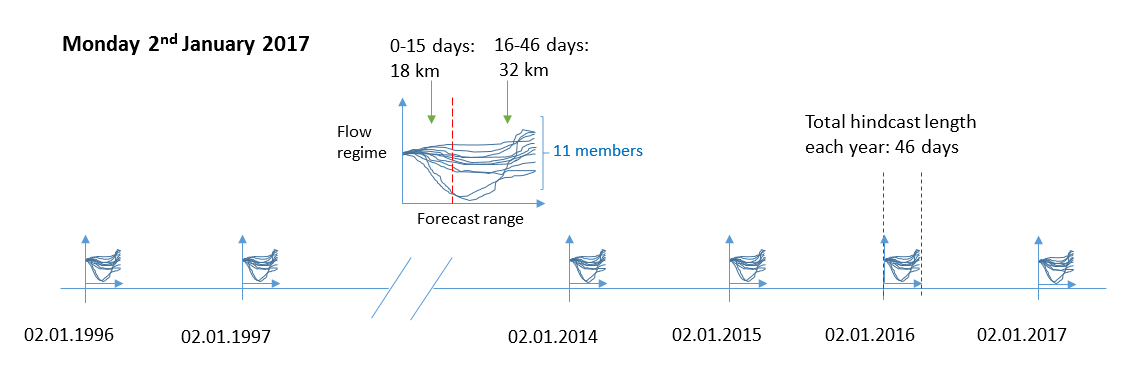
\includegraphics[width=34pc,angle=0]{H:/Documents/Thesis/phd-thesis-template-2.2.2_AC/phd-thesis-template-2.2.2/Figs/ec_hindcast2.png}
	\caption{An example of the ECMWF hindcast schedule. For example, on Monday 2nd January 2017, 20 hindcast years (back to 1996) will be run. Each ensemble is made up of 11 members that reduce in resolution at day 15. (or day 10?) and run for a total of 46 days.}\label{fig:ecmwf_hindcast}
	\centering
\end{figure}

Over a year, with a model run on every Monday and Thursday for ... days, an entire 20 year period with xxx ensembles will have been created.

Hindcasts are a useful product to use......

A hindcast, or reforecast is a model forecast run initialised with conditions in the past. The hindcast run commences every Monday and Thursday, for that day for the past 20 years (to 1996) (figure \ref{fig:hindcast}).


Over a year, with a model run on every Monday and Thursday, an entire 20 year period with 10 ensembles members plus the control will have been created. Resolution of all of the members decreases at day 16. The initial 15 days of the hindcast that are analysed here have a resolution of 0.2$^0$. The ensemble members have five different ocean temperature analyses, with members 1 and 6, 2 and 7, 3 and 8, 4 and 9, 5 and 10 sharing the same initial state. These perturbed states are produced by adding randomly chosen wind perturbations to the ocean data assimilation, driven by five slightly different meteorological fields based on the control analysis.

For the ocean, we use 5 different ocean re-analyses (control + 4 perturbed) which are used to perturb the 11 members - which means that there are pairs of members which share the same SSTs as you said.

atmosphere: Singular vectors are applied in the Extratropics + Ensemble data assimilation (EDA) perturbations everywhere.

No, the atmospheric model is also perturbed using stochastic perturbations (SPPT scheme and also back-scatter scheme for the model version you are using), but only for the perturbed forecasts. The control forecast (type  cf or ensemble 0) is not perturbed. 

(Frederic email 9 Nov)
%What about the different atmosphere or model parts?
%The current version of the ECMWF model is given .. data based on xx of a day in the past and then runs forwards as a forecast. This provides a way to calibrate the output.
%Skill evaluation and calibration - the model drifts, so need to estimate from the model climate. Do not issue forecasts directly from the model, use anomalies.
%Reforecasts initialised from ERA-Interim, not OSTIA.

%% Analysis and model physics perturbed  https://www.ecmwf.int/en/forecasts/documentation-and-support#reforecasts
%ensemble members lower res???  na... all 18 km ??
%


\subsubsection {Operational forecast}  \label{ECMWF_forecast}
The high resolution (deterministic) operational forecast uses an atmosphere-only GCM. SSTs come from the Operational Sea Surface Temperature and Sea Ice Analysis (OSTIA) analysis at day 0, which persist throughout the forecast window (days 0-10). This is a high resolution analysis of the SST for the global ocean with daily, global coverage 1/20$^0$ ($\tilde{6}$ km) combined SST and sea ice concentration product, which is generated in near real time \citep{donlon2012operational}.

\begin{table}%[h]
	\caption{Operational forecast resolution}\label{t_ecmwf2}
	%	\begin{center}
	%	\begin{tabular}{cccccccc} use p to wrap text
	\begin{tabular}{ ccc }
		\hline\hline
		Date & Grid & Horizontal resolution \\
		\hline\hline
		21.11.00 & N256 & 0.5$^0$ \textasciitilde{40} km \\ %% $ $ is math mode - put this around the bits that are not text
		01.02.06 & N400 & 0.225$^0$ \textasciitilde{25} km \\ %% $ $ is math mode - put this around the bits that are not text
		26.01.10 & N640 & 0.125$^0$ \textasciitilde{16} km \\ %% $ $ is math mode - put this around the bits that are not text
		08.03.16 & O1280 & 0.1$^0$ \textasciitilde{9} km \\ %% $ $ is math mode - put this around the bits that are not text		
		\hline
	\end{tabular}
	%\end{center}
\end{table}

The grid used for the operational forecasts is updated every \textasciitilde{6} years and is currently being run at 0.1$^0$ resolution (table \ref{t_ecmwf2}).
%What is the spectral resolution??
%
%The sst and sea ice are updated during the model integration according to the tendency obtained from climatology of OSTIA (5km) \citep{ecmwf_user_guide}.
%
%The ensemble forecast (days 0-10) is at half the horizontal resolution and also has fewer levels in the vertical.  During these initial 10 days, the forecast uses an atmosphere-only GCM, with OSTIA SSTs. Five different ocean analyses are distributed amongst the control and ensemble members, produced by adding wind perturbations from different meteorological fields. \citep{ecmwf_user_guide}.  From days 10-46, the horizontal resolution of the ensemble is reduced to half (to 32 km) and the atmosphere is coupled to the NEMO ocean model \citep{madec2015nemo}. 
%The 50 ensemble members are formed by making small changes to the 4D-VAR analysis, creating perturbed initial states \citep{ecmwf_user_guide}.
%
%How are the ensembles generated - different ocean initial state and atmospheric initial state??
%
%ensemble forecast:
%The horizontal resolution of the ensemble is reduced at day 10, and the remainder of the forecast (out to 15 or 32 days) is run at half the resolution of the first 10 days.
%No ocean coupling for the first 10 days. From day 10 onwards, coupled to ocean model (5 ocean analyses for initial conditions).
%
%
%"The ocean-atmosphere coupling is achieved by a two-way interaction: the atmosphere affects the ocean through its wind, heat and net precipitation (precip-evap), whilst the ocean affects the atmosphere through its SST. for the ENS, this interaction is every hour" \citep{ecmwf_user_guide}.
%
%With respect to synoptic patterns, the control ensemble forecast  gives a similar performance to HRES, which is at twice the resolution \citep{ecmwf_user_guide}. However, HRES is better at forecasting small-scale extreme events, for example strong winds and heavy rain, when resolution is more important. 
%
%The high resolution model will be coupled to NEMO 0.25$^0$ at the end of 2017.
%Verification against ERA-Interim.
%Archived at the resolution run at.


The high resolution (deterministic) operational forecast uses an atmosphere-only GCM. SSTS come from the Operational Sea Surface Temperature and Sea Ice Analysis (OSTIA) analysis at day 0, which persist throughout the forecast window (days 0-10). This is a high resolution analysis of the SST for the global ocean with daily, global coverage 1/20° (~6 km) combined SST and sea ice concentration product, which is generated in near real time \citep{donlon2012operational}.
What is the spectral resolution??

The sst and sea ice are updated during the model integration according to the tendency obtained from climatology of OSTIA (5km) \citep{ecmwf_user_guide}.

The ensemble forecast (days 0-10) is at half the horizontal resolution ( x compared to x) and also has fewer levels in the vertical.  During these initial 10 days, the forecast uses an atmosphere-only GCM, with OSTIA SSTs. Five different ocean analyses are distributed amongst the control and ensemble members, produced by adding wind perturbations from different meteorological fields. \citep{ecmwf_user_guide}.  From days 10-46, the horizontal resolution of the ensemble is reduced to half (to 32 km) and the atmosphere is coupled to the NEMO ocean model \citep{madec2015nemo}. 
The 50 ensemble members are formed by making small changes to the 4D-VAR analysis, creating perturbed initial states \citep{ecmwf_user_guide}.

How are the ensembles generated - different ocean initial state and atmospheric initial state??

ensemble forecast:
The horizontal resolution of the ensemble is reduced at day 10, and the remainder of the forecast (out to 15 or 32 days) is run at half the resolution of the first 10 days.
No ocean coupling for the first 10 days. From day 10 onwards, coupled to ocean model (5 ocean analyses for initial conditions).


"The ocean-atmosphere coupling is achieved by a two-way interaction: the atmosphere affects the ocean through its wind, heat and net precipitation (precip-evap), whilst the ocean affects the atmosphere through its SST. for the ENS, this interaction is every hour" \citep{ecmwf_user_guide}.

With respect to synoptic patterns, the control ensemble forecast  gives a similar performance to HRES, which is at twice the resolution \citep{ecmwf_user_guide}. However, HRES is better at forecasting small-scale extreme events, for example strong winds and heavy rain, when resolution is more important. 

The high resolution model will be coupled to NEMO 0.25$^0$ at the end of 2017.
Verification against ERA-Interim.
Archived at the resolution run at.


\begin{table}%[h]
	\caption{Operational forecast resolution}\label{t_ecmwf2}
	%	\begin{center}
	%	\begin{tabular}{cccccccc} use p to wrap text
	\begin{tabular}{ ccc }
		\hline\hline
		Date & Grid & Horizontal resolution \\
		\hline\hline
		21.11.00 & N256 & 0.5$^0$ \textasciitilde{40} km \\ %% $ $ is math mode - put this around the bits that are not text
		01.02.06 & N400 & 0.225$^0$ \textasciitilde{25} km \\ %% $ $ is math mode - put this around the bits that are not text
		26.01.10 & N640 & 0.125$^0$ \textasciitilde{16} km \\ %% $ $ is math mode - put this around the bits that are not text
		08.03.16 & O1280 & 0.1$^0$ \textasciitilde{9} km \\ %% $ $ is math mode - put this around the bits that are not text		
		\hline
	\end{tabular}
	%\end{center}
\end{table}

The grid used for the operational forecasts is updated every \textasciitilde{6} years and is currently being run at 0.1$^0$ resolution (table \ref{t_ecmwf2}).
%What is the spectral resolution??
%
%The sst and sea ice are updated during the model integration according to the tendency obtained from climatology of OSTIA (5km) \citep{ecmwf_user_guide}.
%
%The ensemble forecast (days 0-10) is at half the horizontal resolution and also has fewer levels in the vertical.  During these initial 10 days, the forecast uses an atmosphere-only GCM, with OSTIA SSTs. Five different ocean analyses are distributed amongst the control and ensemble members, produced by adding wind perturbations from different meteorological fields. \citep{ecmwf_user_guide}.  From days 10-46, the horizontal resolution of the ensemble is reduced to half (to 32 km) and the atmosphere is coupled to the NEMO ocean model \citep{madec2015nemo}. 
%The 50 ensemble members are formed by making small changes to the 4D-VAR analysis, creating perturbed initial states \citep{ecmwf_user_guide}.
%
%How are the ensembles generated - different ocean initial state and atmospheric initial state??
%
%ensemble forecast:
%The horizontal resolution of the ensemble is reduced at day 10, and the remainder of the forecast (out to 15 or 32 days) is run at half the resolution of the first 10 days.
%No ocean coupling for the first 10 days. From day 10 onwards, coupled to ocean model (5 ocean analyses for initial conditions).
%
%
%"The ocean-atmosphere coupling is achieved by a two-way interaction: the atmosphere affects the ocean through its wind, heat and net precipitation (precip-evap), whilst the ocean affects the atmosphere through its SST. for the ENS, this interaction is every hour" \citep{ecmwf_user_guide}.
%
%With respect to synoptic patterns, the control ensemble forecast  gives a similar performance to HRES, which is at twice the resolution \citep{ecmwf_user_guide}. However, HRES is better at forecasting small-scale extreme events, for example strong winds and heavy rain, when resolution is more important. 
%
%The high resolution model will be coupled to NEMO 0.25$^0$ at the end of 2017.
%Verification against ERA-Interim.
%Archived at the resolution run at.

\subsubsection {ERA-Interim reanalysis}  \label{ECMWF_ERA}
 

\begin{table}[h]
	\caption{Variables}\label{t_variables}
	\begin{center}
		\begin{tabular}{ccc}

			\hline\hline
			$Variable$ & $Units$ & $Pressure Levels (hPa)$ \\
			\hline
			Zonal wind (u) & ms$^-1$ & 300, 400, 500, 700, 850, 925, 1000 \\ %% $ $ is math mode - put this around the bits that are not text
			Meridional wind (v) & ms$^-1$ & 300, 400, 500, 700, 850, 925, 1000  \\
			Vertical .. (w) & ms$^-1$ & 300, 400, 500, 700, 850, 925, 1000  \\
			Temperature (t) & K & 300, 400, 500, 700, 850, 925, 1000 \\
			Potential temperature (theta) & ms & 300, 400, 500, 700, 850, 925, 1000  \\
			q (q) & ms & 300, 400, 500, 700, 850, 925, 1000  \\
			Potential vorticity (PV) & ms & N/A  \\
			Geopotential height (Z) & ms & xx  \\

			\hline
		\end{tabular}
	\end{center}
\end{table}
% available at 50, 100, 200, 300, 400, 500, 700, 850, 925, 1000
Specific Humidity, Quasi-geostrophic Potential Vorticity, Water Vapor Mixing Ratio

At 6-hourly temporal resolution, time step 0 to 360, which is 10 days.

ERA-Interim is a global atmospheric reanalysis from 1979, continuously updated in real time. The spatial resolution of the data set is approximately 80 km (T255 spectral) on 60 vertical levels from the surface up to 0.1 hPa \citep{dee2011era}.

%http://www.ecmwf.int/en/research/modelling-and-prediction/atmospheric-dynamics
%"The wave model at ECMWF is called the “WAM”. It describes the rate of change of the 2- dimensional wave spectrum, in any water depth, caused by advection, wind input, dissipation due to white capping and bottom friction and non-linear wave interactions. It is set up so as to allow the two-way interaction of wind and waves with the atmospheric model. It is also incorporated in the medium-range, monthly and seasonal ensembles. 
%Radar altimeter wave-height data are assimilated from satellites. Buoy wave data are not assimilated; instead, they serve as an independent check on the quality of modelled wave parameters. The propagation of swell in the wave model is handled by a simple scheme that gives rise to a smoothing of the wave field. At present the effects of surface currents on the sea state are not taken into account. In particular areas, such as the Gulf Stream or Agulhas current, the current effect may give rise to localised changes of up to one metre in the wave height. The representation of the sea-ice fields is not as accurate as would be needed to handle waves near the ice edge. Due to the present model resolution, wave products near the coasts and, to a lesser extent, in small enclosed basins (e.g. the Baltic Sea) may be of lower quality than the open-ocean products. "
%Tides?

"The OGCM can reproduce the general features of the circulation and the thermal structure of the upper layers of the ocean and its seasonal, but has systematic errors, some of which are caused by the coarse vertical and horizontal resolution: the model thermocline is too diffuse; the Gulf Stream does not separate at the right location. (ref online guide).
The ocean analysis is performed every 10 days, down to a depth of 2000 m. The ocean-atmosphere coupling is achieved by a two-way interaction: the atmosphere affects the ocean through its wind, heat and net precipitation (precipitation-evaporation), whilst the ocean affects the atmosphere through its SST. For ENS, this interaction is every hour. what about regular forecast? not needed?? "


\begin{figure}
	
	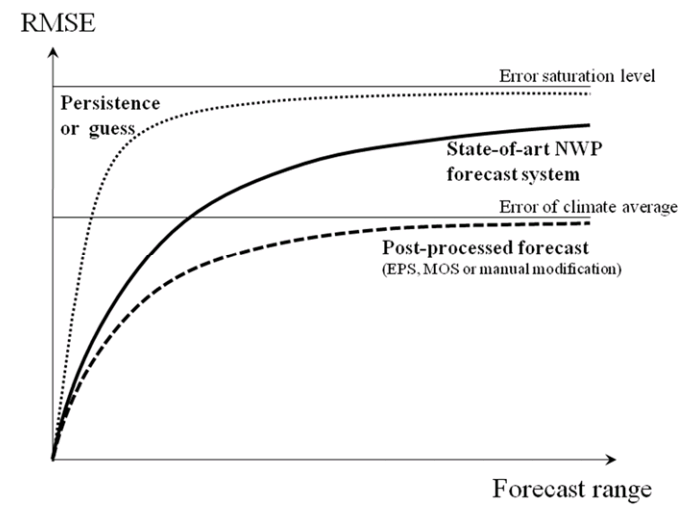
\includegraphics[width=22pc,angle=0]{H:/Documents/Thesis/phd-thesis-template-2.2.2_AC/phd-thesis-template-2.2.2/Figs/forecast_error.png}
	\caption{Forecast error. From ECMWF web guide}\label{fig:forecast_error}
	\centering
\end{figure}


More details about spectral and truncation. Spectral and grids...
Parametrisation scheme...
global
hydrostatic - pressure coordinates?

%I will be looking at the medium-range(3-10 days). ECMWF’s forecasts cover time frames ranging from medium-range (3-10 days), to monthly and seasonal, and up to a year ahead.
%Nowcasting (0 - 6 hours)
%Short-range weather forecasts (1 - 3 days)
%Medium-range weather forecasts (3 - 10 days)

%"Between day 9 and day 10 there is a 24-hour overlap period, to reduce the “shock” of the change, in particular for the parameters that are most sensitive, for example convection and large-scale precipitation. Accumulations of precipitation (and other fluxes) for periods that span the resolution change (day 10) need to use low-resolution data from the overlap period and such data is thereforeavailable via dissemination."

%Not dealt with 'Forecasts from 15 to 32 days'

ERA-5 reanalysis download at 0.25 degree resolution
https://software.ecmwf.int/wiki/display/CKB/ERA5+data+documentation

% https://software.ecmwf.int/wiki/display/CKB/Does+downloading+data+at+higher+resolution+improve+the+output

For ERA-Interim the point interval on the native Gaussian grid is about 0.75 degrees (with the exception of Ocean-Wave data which are natively stored on the wave model’s reduced 1.0x1.0 degrees latitude/longitude grid). You can specify a custom grid on the data server web interface, or using the ECMWF WebAPI or using the MARS client (if you have access to it).  On the web interface the default grid for ERA-Interim is lat/long, with a default resolution of 0.75x0.75 degrees (about 80km), approximating the irregular grid spacing on the native Gaussian grid.

For ERA5 data the point interval on the native Gaussian grid is about 0.28 degrees. You can download ERA5 data using Python and specify a custom grid and resolution in your script. You should set the horizontal resolution to slightly lower than 0.28 degrees (about 30km), for example to 0.25 degrees, approximating the irregular grid spacing on the native Gaussian grid.



\subsection{Ensemble forecasting}

A hindcast, or reforecast is a model forecast run initialised with conditions in the past. The hindcast run commences every Monday and Thursday, for that day for the past 20 years (to 1996) (figure \ref{fig:hindcast}).

\begin{figure} [h]
	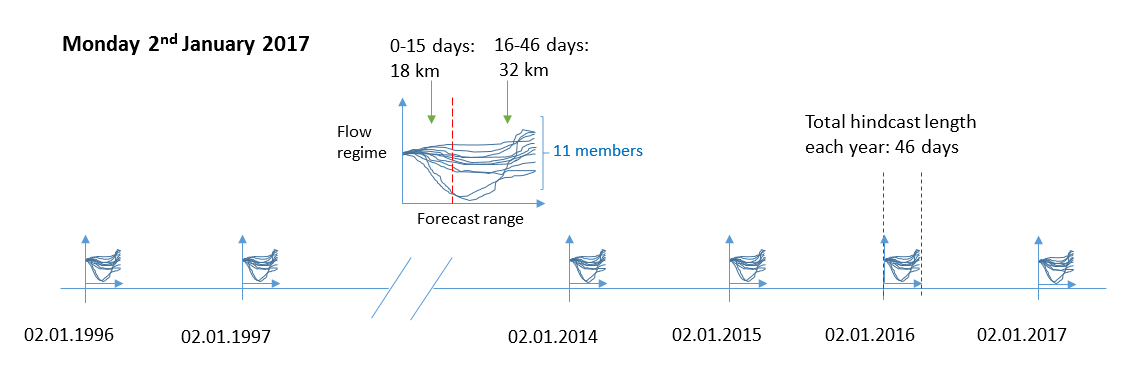
\includegraphics[width=34pc,angle=0]{H:/Documents/Thesis/phd-thesis-template-2.2.2_AC/phd-thesis-template-2.2.2/Figs/ec_hindcast2.png}
	\caption{An example of the ECMWF hindcast schedule. For example, on Monday 2nd January 2017, 20 hindcast years (back to 1996) will be run. Each ensemble is made up of 11 members that reduce in resolution at day 15 and run for a total of 46 days.}\label{fig:ecmwf_hindcast}
	\centering
\end{figure} \label{fig:hindcast}	

Over a year, with a model run on every Monday and Thursday, an entire 20 year period with 10 ensembles members plus the control will have been created. Resolution of all of the members decreases at day 16. The initial 15 days of the hindcast that are analysed here have a resolution of 0.2$^0$. The ensemble members have five different ocean temperature analyses, with members 1 and 6, 2 and 7, 3 and 8, 4 and 9, 5 and 10 sharing the same initial state. These perturbed states are produced by adding randomly chosen wind perturbations to the ocean data assimilation, driven by five slightly different meteorological fields based on the control analysis.

For the ocean, we use 5 different ocean re-analyses (control + 4 perturbed) which are used to perturb the 11 members - which means that there are pairs of members which share the same SSTs as you said.

atmosphere: Singular vectors are applied in the Extratropics + Ensemble data assimilation (EDA) perturbations everywhere.

No, the atmospheric model is also perturbed using stochastic perturbations (SPPT scheme and also back-scatter scheme for the model version you are using), but only for the perturbed forecasts. The control forecast (type  cf or ensemble 0) is not perturbed. 

(Frederic email 9 Nov)
%What about the different atmosphere or model parts?
%The current version of the ECMWF model is given .. data based on xx of a day in the past and then runs forwards as a forecast. This provides a way to calibrate the output.
%Skill evaluation and calibration - the model drifts, so need to estimate from the model climate. Do not issue forecasts directly from the model, use anomalies.
%Reforecasts initialised from ERA-Interim, not OSTIA.

%% Analysis and model physics perturbed  https://www.ecmwf.int/en/forecasts/documentation-and-support#reforecasts
%ensemble members lower res???  na... all 18 km ??
%
%Hindcasts are a useful product to use......


Poor forecasts result from errors in initial conditions and model errors, with initial conditions dominating during the first five days or so. "Analysis errors amplify most easily in the sensitive parts of the
atmosphere, in particular where strong baroclinic systems develop. These errors then move
downstream and amplify and thereby affect the large-scale flow. To estimate the effect of
possible initial analysis errors and the consequent uncertainty of the forecasts, small changes
to the 4D-Var analysis are made, creating an ensemble of many (currently 50) different,
“perturbed”, initial states. Model deficiencies are represented by a stochastic process. In order
to save computational time, the ensemble members are run with a lower resolution version of
the IFS. 
If the ensembles agree, it is a predictable state. If diverge significantly from each other and the control, less certain forecast. Also calculate the ensemble mean (EM). ENS provides information from which the probability of alternative
developments is calculated, in particular those related to risk of extreme or high-impact
weather. The three methods for creating the ensemble...

%\begin{figure}
%	
%	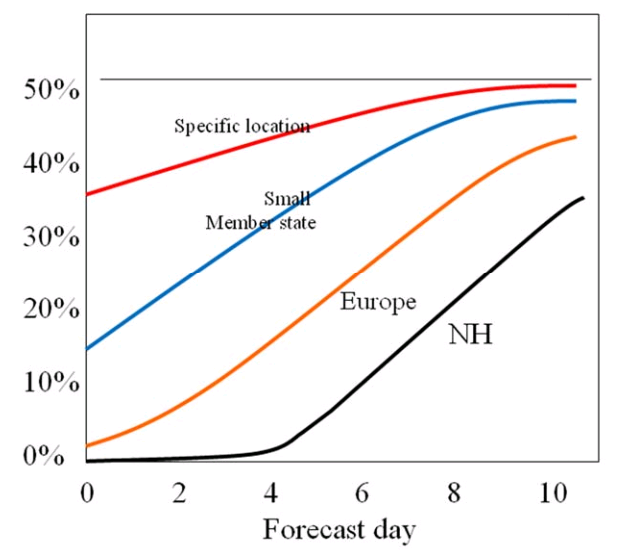
\includegraphics[width=22pc,angle=0]{H:/Documents/Thesis/phd-thesis-template-2.2.2_AC/phd-thesis-template-2.2.2/Figs/ens_pert.png}
%	\caption{Ensemble perturbation}\label{fig:ens_pert}
%	\centering
%\end{figure}

\begin{figure}
	
	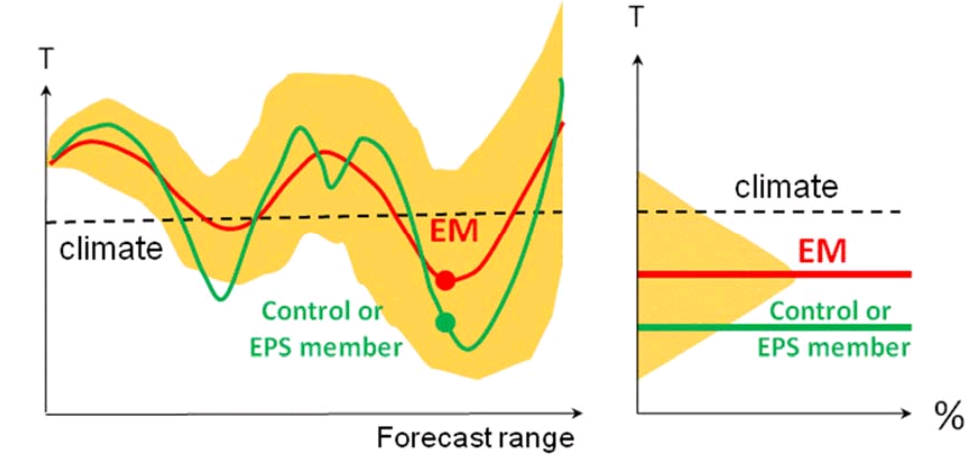
\includegraphics[width=22pc,angle=0]{H:/Documents/Thesis/phd-thesis-template-2.2.2_AC/phd-thesis-template-2.2.2/Figs/ens_spread.png}
	\caption{Ensemble spread}\label{fig:ens_spread}
	\centering
\end{figure}

minobe2010atmospheric
kelly2010western
kwon2010role
Molteni, Corti, Palmer, Mike Wallace

%\subsection{The North Atlantic Oscillation}


\subsubsection {ERA5 reanalysis}  \label{ECMWF_ERA5}
% https://software.ecmwf.int/wiki/display/CKB/What+is+ERA5
ERA5 is the 5th major global reanalysis produced by ECMWF.
ERA5 uses the same 37 pressure levels as ERA-Interim.
All parameters available in ERA-Interim are also available in ERA5; and ERA5 has some additional parameters.
10 ensemble members, and also ensemble mean and spread for all parameters and levels are being produced. The temporal resolution is 3-hourly, rather than hourly for the deterministic ERA5 product, though.

%%%%%%%%%%%%%%%%%%%%%%%%%%%%%%%%%%%%%%%%%%%%%%%%%%%%%%%%%%%%%%%%%%%%%%

\chapter {Research question (Thesis chapter 2)} \label{Ch2}

Many authors have emphasised the importance of shear (symmetric) instability in extra-tropical cyclones, namely in relation to precipitation bands. However, much of this work has been based on theory and little has been done to explore this mechanism in model forecasts. Here, I examine a single storm in a suite of model runs and compare results to theory.

\section{Aims}
\begin{itemize}
	\item Diagnose shear instability in a suite of model runs for an extra-tropical cyclone around 15th January 2004 over the Gulf Stream
	\item Explore the relationship of the shear instability with other variables, including precipitation
	\item Analyse atmospheric structure and characteristics that generate shear instability
	\item Examine differences between different model runs within same the resolution ensemble and also compare with members of different resolution
\end{itemize}

This storm on 15th January 2004 has been chosen as it has previously been used to show that the Gulf Stream is important \citep{sheldon2017warm}. 

%Total precipitation is comprised of convective precipitation and large scale (stratiform) precipitation. Convective precipitation produced by the convection scheme.


\section {Method}  \label{method}

Ensemble forecast hindcast data that is initialised on 12th January 2017 and set up with 12th January 2004 conditions was used. The vertical velocity data ($\omega$, Pa/s) is only complete at 12 hourly time steps and so the shear diagnostic could only be computed at 00 and 12 UTC. The storm developed over the Gulf Stream on 12 UTC 15th January, and so analysis is from initialisation + 4 days (96 hours).
%#, so expect the members to have diverged.
%
%Initial analysis based around establishing whether the shear instability seen in \cite{sheldon2017warm} in MetUM is also apparent in the ECMWF hindcast dataset. 
%
%Hindcast analysis is from the hindcast initialised on 00 UTC 12th January, so a lead time of at least +84 hours for the first time shown. Met Office was initialised 12 UTC 14th, so lead time of 24 hours only.


%Land mask

A spatial low pass and high pass filter was applied to the original data to obtain the small scale (${\omega}$', u', v') and mean ($\overline{w}$, $\overline{u}$, $\overline{v}$) values. An average over approximately 150 km in each direction for each point was calculated. Using 150 km allows for a low pass for ERA-Interim to be calculated, which is 0.75$^0$ resolution. The high pass, to capture the high frequency variability, was calculated by subtracting the low pass from the original field. This is to separate the low frequency background from the high frequency perturbations.
% which is comparable to the Met Office experiment \cite{sheldon2017warm}, where 120 km in each direction was used.

\begin{table}
	\caption{Low pass filter dimensions for different products}\label{t_lowpass}
	\begin{center}
		\begin{tabular}{cccc}
			%	\begin{tabular}{ | m{3.0cm} | m{2cm}| m{1.2cm} | m{2cm}| }
			\hline\hline
			Product & Resolution & No. grid points in each direction & Low pass scale \\
			\hline
			Hindcast & 0.2 & 7 & 140 km \\ 
			ERA-Interim & 0.75  & 2 & 150 km \\
			Forecast (2004) & 0.5 &  3 & 140 km \\ %%%%%%%%%% check			
			
			\hline
		\end{tabular}
	\end{center}
\end{table}


\begin{figure}
	\centering	
	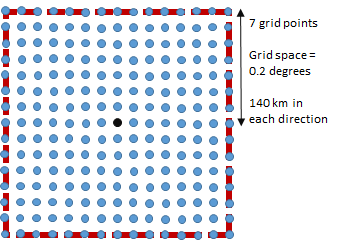
\includegraphics[width=16pc,angle=0]{H:/Documents/Thesis/phd-thesis-template-2.2.2_AC/phd-thesis-template-2.2.2/Figs/low_pass.png}
	\caption{Domain used to create the low pass for the hindcast data.  The hindcast data is at 0.2 degree resolution and so the domain used is 1.4 degrees in each direction, approximately 140 km. At each grid point, all values within this domain are averaged to create the low pass at that point.}\label{fig:low_pass}
	\centering
\end{figure}

The shear diagnostic was computed using equation \ref{eq_diag} at the 500 hPa level.
%, which is comparable to the 5 km used in the Met Office analysis.

%The storm characteristics were different for the different members in term of location and intensity and so for each member, a rectangular domain around the storm minimum central pressure was computed, moving with the storm at each time step. The domain extends to the south and west of the low pressure centre, in order to capture the frontal activity?
%Histograms of variables within this domain were produced (number of datapoints).
%
%Other variables including precipitation, etc. also analysed using the same low pressure following domain.
%Eddy Kinetic energy also calculated and buoyancy diagnostic
%
%Table of diagnostics and other variables.
%
%The potential vorticity (PV) data in the ECMWF forecast hindcast is only available on the 320 isentropic level. 
%
%Analysis produced at the four main synoptic hours 00, 06, 12 and 18 UTC. They are the best gridded estimate of the state of the atmosphere (best fit to observations). 
%Forecast based on the 00/12 UTC Analysis. Meteorological parameters are written output for every forecast time step, 3-hourly intervals from 00 to 72 hours, and 6-hourly from 72 to 240 hours. Forecast 0 hr is same as analysis.

 general stuff about preparing the data, interpolating levels?
Ensemble forecast hindcast data was used, with 'refdate' 12/01/2017, date of real-time forecast associated to re-forecast/hindcast, and 'hdate' 12/01/2004, base date of a hindcast. Initial analysis based around establishing whether the shear instability seen in (paper) in met office model is also apparent in the ECMWF hindcast dataset. 
The date of the following hindcast was 16/01/2007. The Met Office analysis ran from UTC 14/01/2004 and focussed on +24 hours, at ...
This analysis has a longer lead time (by 24 hours?) to the analysis time. At 12 UTC on 15th January, the storm had started to develop but was slower, less intense than the Met Office simulation. Therefore the main analysis time is 00UTC on 16th and the following two time steps.
The vertical velocity data ($\omega$, Pa/s) is only complete at 12 hourly time steps and so the diagnostic could only be computed at 00 and 12 UTC.


Land mask

\subsection {PV and momentum flux diagnostics}

The shear instability diagnostic:

\begin{equation} \label{eq_diag}
-\overline{w'u'} . \frac{\overline{\partial u}}{\partial z}
\end{equation}


% dubar/dp x (u'w')bar + dvbar/d[ x (v'w')bar
\begin{equation} \label{eq_diag1}
-\overline{w'u'} . \frac{\partial{\overline u}}{\partial z} + \overline{w'v'} . \frac{\partial{\overline v}}{\partial z}
\end{equation}

\begin{equation} \label{eq_diag2}
\frac{\partial}{\partial{t}} EKE = -\overline{w'u'} . \frac{\partial{\overline u}}{\partial z} + \overline{w'v'} . \frac{\partial{\overline v}}{\partial z} + ...
\end{equation}

NOTE: in calculating buoyancy, must take the low pass. This shows a mean spatial field. This is because it shows you that the small scale perturbations are having an effect on the large scale. If they evened out, the mean would be zero. This is also the case when take the low pass of the diagnostic.

% From Tellus warm path paper: To do so, we have applied spatial low-pass and high-pass filters on the 12 km grid (these were simply obtained by averaging at each point the 10 neighbouring points – separated by approximately 12 km so overall an average over 240 km – in the zonal and meridional directions, the ‘lowpass’, and then removing this average, the ‘high-pass’).  GIVES +120 in each direction for MO. I used +150 so that could do 2x0.75 for ERA

A spatial low pass and high pass filter was applied to the original data to obtain the prime' values (w', u', v') and bar values. An average over approximately 150 km in each direction for each point was calculated, which is comparable to the Met Office, where 120 km in each direction was used. In this case, using 150 km allows for a low pass for ERA-Interim to be calculated, which is 0.75 resolution. The high pass, to capture the high variability, was original minus low pass. This is to separate the low frequency background from the high frequency perturbations.


\begin{table}[h]
	\caption{Low pass filter dimensions for different products}\label{t_lowpass}
	\begin{center}
		\begin{tabular}{cccc}
	%	\begin{tabular}{ | m{3.0cm} | m{2cm}| m{1.2cm} | m{2cm}| }
			\hline\hline
			Product & Resolution & No. grid points in each direction & Low pass scale \\
			\hline
			Hindcast & 0.2 & 14 & 140 km \\ 
			ERA-Interim & 0.75  & 2 & 150 km \\
			Forecast & Variable &  x & x \\			
			
			\hline
		\end{tabular}
	\end{center}
\end{table}


\begin{figure}
	
	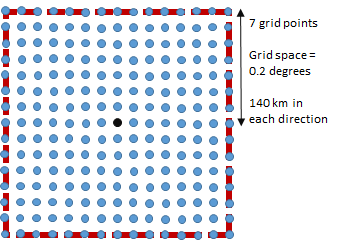
\includegraphics[width=16pc,angle=0]{H:/Documents/Thesis/phd-thesis-template-2.2.2_AC/phd-thesis-template-2.2.2/Figs/low_pass.png}
	\caption{Domain used to create the low pass for the hindcast data.  The hindcast data is at 0.2 degree resolution and so the domain used is 1.4 degrees in each direction, approximately 140 km. At each grid point, all values within this domain are average to create the low pass at that point. ERA Interim has grid spacing f 0.75 degrees and so a low pass using 2 points in each direction was used (1.5 degrees). For the winter hindcast at 0.1 degree spacing, 14 grid points in each direction were used.}\label{fig:low_pass}
	\centering
\end{figure}


The 500 hPa level was analysed, which is comparable to the 5 km used in the Met Office analysis, and shear between levels used 600-400 hPa shear.

The storm characteristics were different for the different members in term of location and intensity and so for each member, a rectangular domain around the storm minimum central pressure was computed, moving with the storm at each time step. The domain extends to the south and west of the low pressure centre, in order to capture the frontal activity?
Histograms of variables within this domain were produced (number of datapoints).

Other variables including precipitation, etc. also analysed using the same low pressure following domain.
Eddy Kinetic energy also calculated:

\begin{equation} \label{eq_EKE}
\frac{\overline{(u'^{2}+v'^{2})}}{2} 
\end{equation}

The potential vorticity (PV) data in the ECMWF forecast hindcast is only available on the 320 isentropic level. 

Analysis produced at the four main synoptic hours 00, 06, 12 and 18 UTC. They are the best gridded estimate of the state of the atmosphere (best fit to observations). 
Forecast based on the 00/12 UTC Analysis. Meteorological parameters are written output for every forecast time step, 3-hourly intervals from 00 to 72 hours, and 6-hourly from 72 to 240 hours. Forecast 0 hr is same as analysis.

Pairs of ensemble members have the same SST field (member1\&6, member2\&7, member 3\&8, member 4\&9, member 5\&10)


\begin{figure}
	
	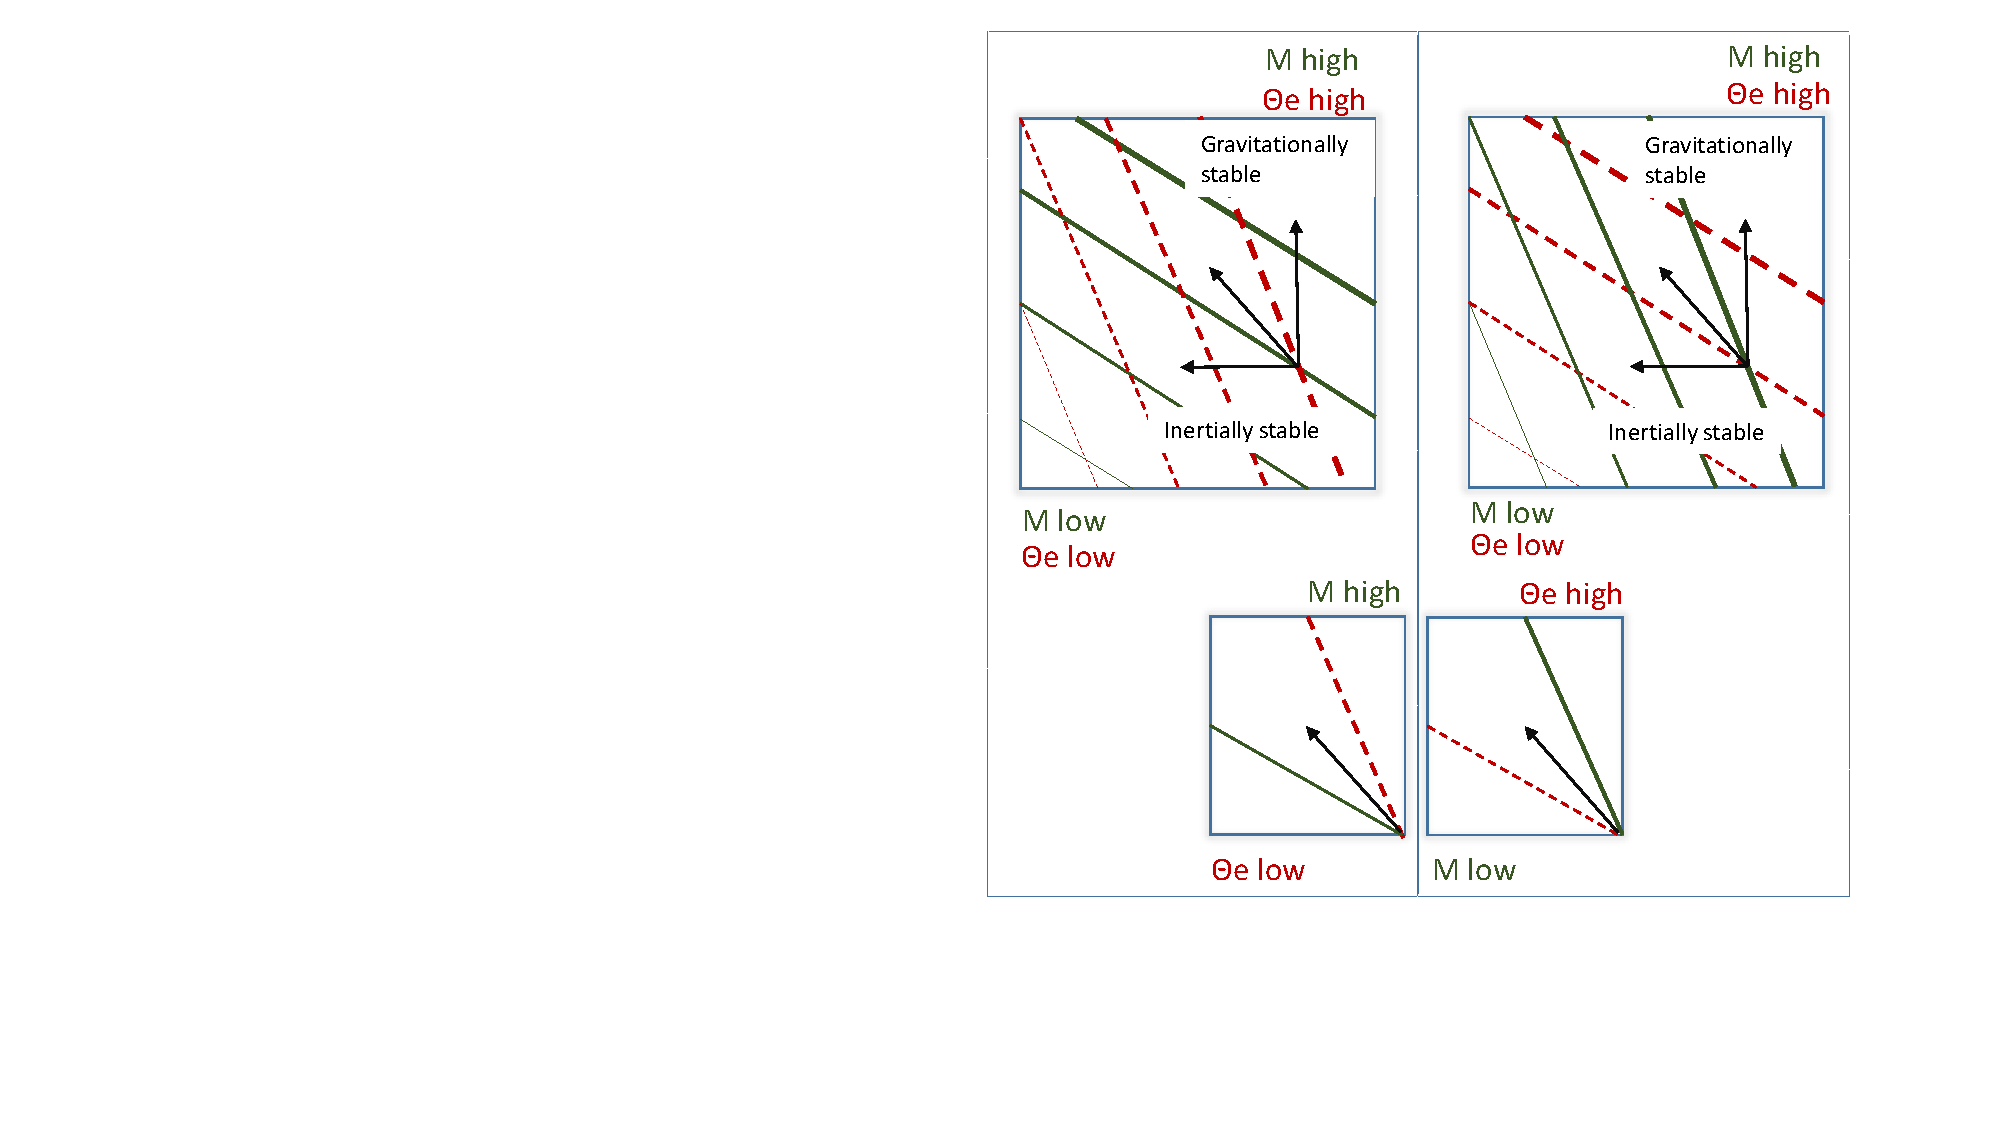
\includegraphics[width=38pc,angle=0]{H:/Documents/Thesis/phd-thesis-template-2.2.2_AC/phd-thesis-template-2.2.2/Figs/mocrette_diagram.pdf}
	\caption{Symmetric instability. (what plane, ie x and z). Lines of constant equivalent potential temperature (theta e)  are shown in read dashed lines and lines of constant angular momentum (M) in solid green. Thickness of the lines increases towards  higher values. Both environments are baroclinic and theta e and M are low in the bottom left and high in the top right. The black arrows show direction of movement of air parcels. In both panels a and b, if a panel is moved to the left, it is inertially stable as it is moving towards an area of reduced angular momentum. Both panels, if a parcel is moved vertically, they are gravitationally stable as potential temperature is increasing. If an air parcel is moved along arrow x in a, it is moving towards lower potential temperature and high M, so . In the other case, it will move towards high theta e and low M, and so. Modified from \cite{morcrette2004radar}}\label{fig:symm_inst}
	\centering
\end{figure}


\begin{figure}
	
	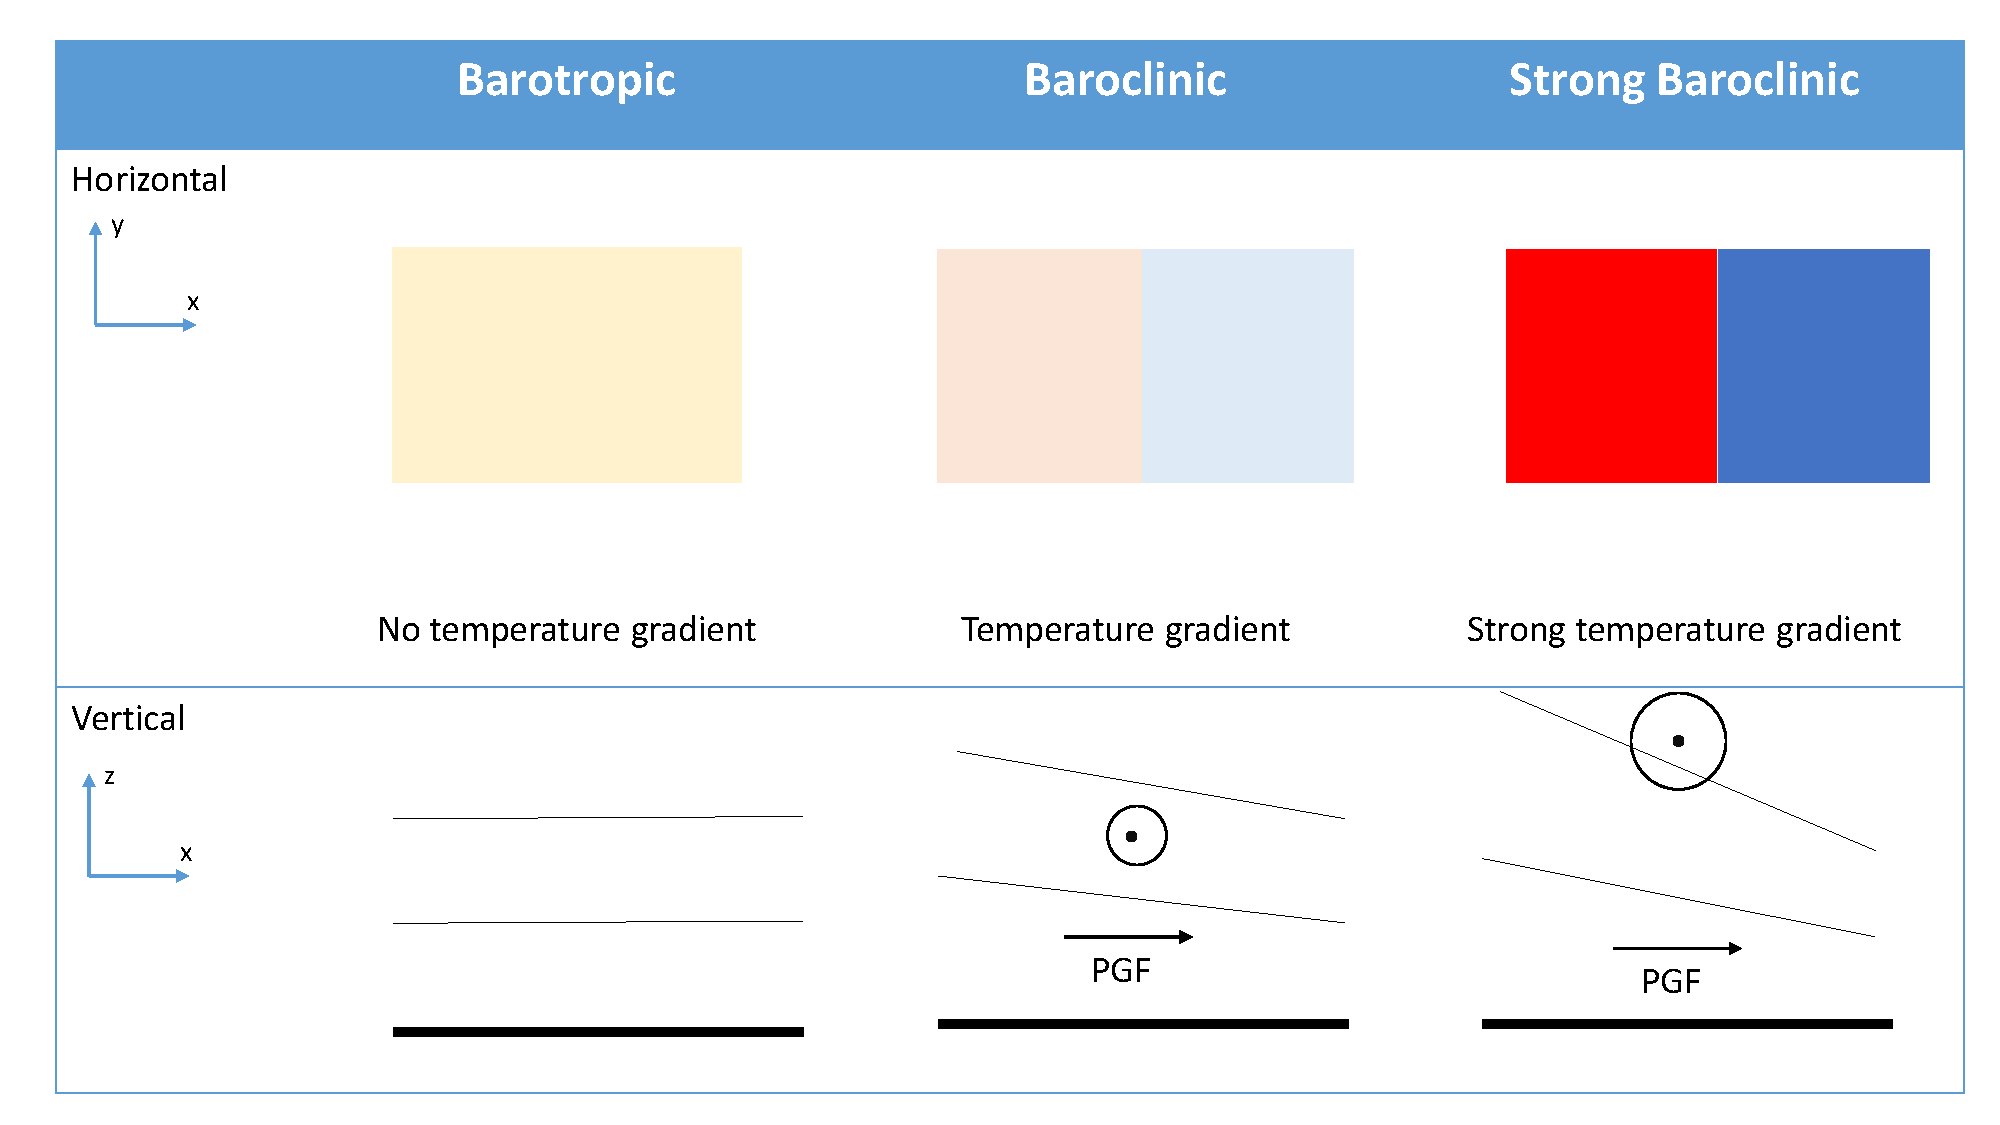
\includegraphics[width=34pc,angle=0]{H:/Documents/Thesis/phd-thesis-template-2.2.2_AC/phd-thesis-template-2.2.2/Figs/barotropic2.pdf}
	\caption{Barotropic and baroclinic environments in the horizontal and vertical, and resultant pressure gradient force and thermal wind.}\label{fig:barotropic}
	\centering
\end{figure}

The high resolution single forecast was analysed for December 2016-February 2017. This is 9 km and downloaded on 0.1 degree resolution. Used 14 points for low pass

Buoyancy (b). g is acceleration due to gravity \(9.8ms^{-1}\). {\rho} is density.

\begin{equation} \label{eq_b}
b = -g\frac{\rho}{\rho_0}
\end{equation}

Total precipitation is comprised of convective precipitation and large scale (stratiform) precipitation. Convective precipitation produced by the convection scheme. 

Potential temperature is a more useful quantity than temperature as it is not affected my vertical movements - expansion and compression of air mass. Also most unstable path? requires no buoyancy. Calculated from temperature and pressure

% used to use the brackets and backslash. Now use equation environment \[\theta =  T \big(\frac{P_0}{P}) ^{0.286} \]
\begin{equation} \label{eq_theta}
\theta =  T \big(\frac{P_0}{P}) ^{0.286}
\end{equation}

Also calculated upright buoyancy (w'{\alpha})

\section{Results}

Results show analysis in the horizontal and vertical of a single extra-tropical cyclone from 15th January 12 UTC to 17th January 00 UTC. 

\subsection{Analysis in latitude/longitude plane}

\begin{figure}
	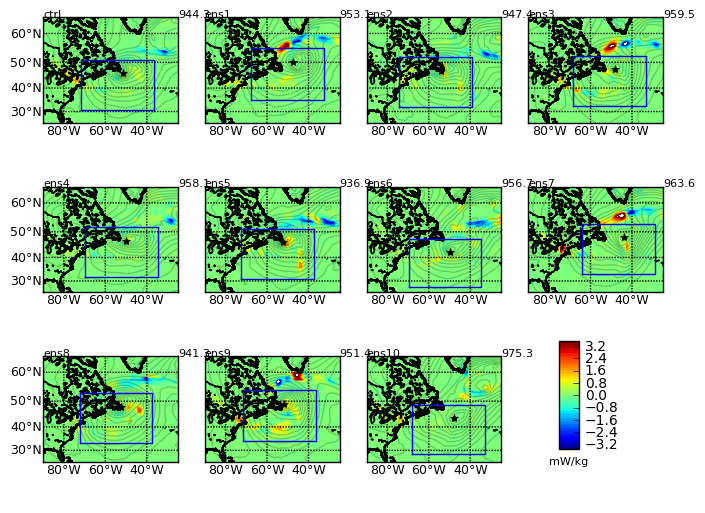
\includegraphics[width=42pc,angle=0]{Y:/Code_Data/Chapter2_3/Plots/Jan04_storm/HC_120104/plot_var_poly_all_diag500_msl_00UTC_17.png}
	\caption{Mean sea level pressure (contours) and shear diagnostic (filled contours) for all hindcast members at 00 UTC 17th January 2004. The centre of this low pressure system is marked with a *. The member name is given on the top left of the plot and the minimum pressure on the top right (in hPa). }\label{fig:HC_all}
\end{figure}

Figure \ref{fig:HC_all} shows the shear diagnostic and mean sea level pressure contours at 00 UTC on 17th January (+114 hours) in the hindcast control and 10 members. All of the runs simulate a cyclone, but with different characteristics, for example minimum central pressure and location. The shear diagnostic is resolved in all of the runs, although there are large differences in intensity. The shear diagnostic is generally associated with fronts, which mark the boundary of warm and cold air masses within with the cyclone. Such fronts can be identified by kinks in the isobars and also temperature analysis, with warm air behind the warm front and cold air behind the cold front, with a steep gradient in temperature observed at each front.

The following analysis focusses on ensemble member 9, as this run exhibits a relatively strong diagnostic, which is aligned in such a way that makes it suitable for cross-section analysis (section \ref{cx_analysis}).

\begin{figure}[h]
	\centering
	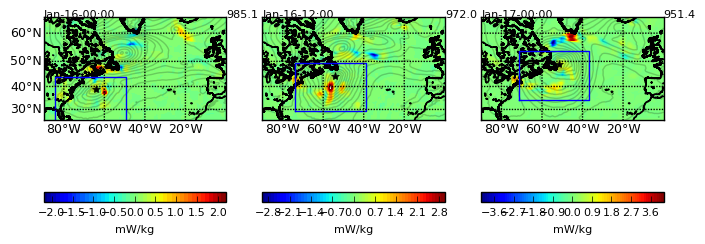
\includegraphics[width=34pc,angle=0]{Y:/Code_Data/Chapter2_3/Plots/Jan04_storm/HC_120104/plot_var_poly_ens9_diag500_msl_12UTC_15_3cb.png}
	\caption{Mean sea level pressure (contours) and diagnostic (filled contours) for hindcast ensemble member 9 at 12 UTC 15th, 00 UTC 16th, 12 UTC 16th January 2004.The centre of this low pressure system is marked with a *. The time is on the top left of the plot and the minimum pressure on the top right (in hPa)}\label{fig:HC_ens9}
	\centering
\end{figure}

Figure \ref{fig:HC_ens9} shows the evolution of ensemble 9 from 00 UTC 16th, with 12-hourly time steps. As the storm deepens and moves north-eastwards, the shear diagnostic increases in intensity. The shear diagnostic also follows the regions of strong gradient in potential temperature, as seen in figure \ref{fig:HC_ens9_pt_RH_precip}, marking cold and warm fronts. Figure \ref{fig:HC_ens9_pt_RH_precip} also shows relative humidity at 500 hPa and precipitation for the 12 hours centred on the time. Moist air is present in the warm sector and the the cold air advected in behind the cold front is relatively dry. The precipitation is intense in the storm centre and along the fronts, especially the trailing cold front, where the sinking cold air is forcing the moist, warm air to ascend.


\begin{figure}	%%% remove [h] here and plots fell into place
	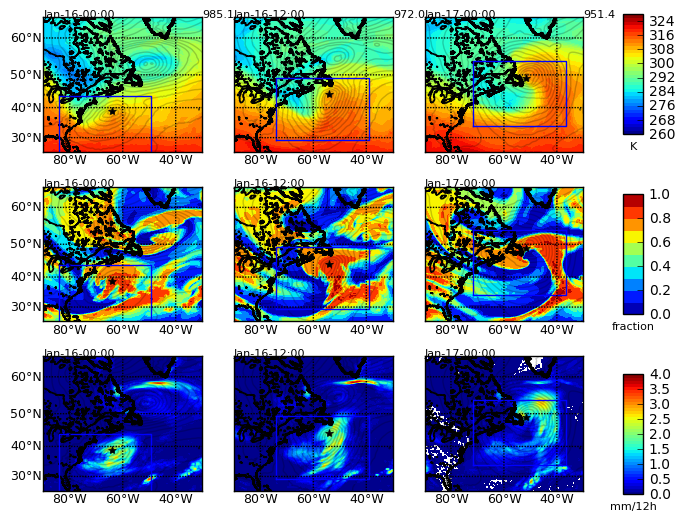
\includegraphics[width=36pc,angle=0]{Y:/Code_Data/Chapter2_3/Plots/Jan04_storm/HC_120104/plot_var_poly_ens9_ptRHprecip_12UTC_15.png}
	\caption{Filled contours: Top panels: 500 hPa potential temperature. Middle panels: 500 hPa relative humidity. Bottom panels: 12-hour precipitation centred on time. Mean sea level pressure is shown in contour line. Hindcast ensemble member 9 at 12 UTC 15th, 00 UTC 16th, 12 UTC 16th January 2004. The centre of this low pressure system is marked with a *. The time is on the top left of the plot and the minimum pressure on the top right (in hPa)}\label{fig:HC_ens9_pt_RH_precip}
	\centering
\end{figure}


%Plots of diag with precip contours overlaid
%\begin{figure}	[h]
%	\includegraphics[width=28pc,angle=0]{Y:/Code_Data/Chapter2_3/Plots/Jan04_storm/HC_120104/plot_var_poly_ens9_diag_precip_12UTC_15.png}
%	\caption{Diagnostic and precip 12 UTC 16th ens9}\label{fig:HC_diag_precip}
%	\centering
%\end{figure}

These results from the hindcast are compared to the coarser ERA-Interim analysis at the same time. The low pass of ERA-Interim was calculated using just two grid points in each direction, as the spacing is much coarser at 0.75 degrees. The shear diagnostic for this same storm is shown in figure \ref{fig:ERA_diag}. The scale is an order of magnitude smaller than figure \ref{fig:HC_ens9}, where hindcast members were 0.2 degrees resolution. During these three time steps, the minimum central pressure is deeper in ERA-Interim than the hindcast ensemble member 9 (970, 952, 948 compared to 985, 972, 951 hPa). However, this is likely due to the timing of the storm system and the higher resolution hindcast member is deepening at a faster rate than the ERA-Interim run. The variables in figure \ref{fig:ERA_pt_RH_precip} show similar characteristics to that for ensemble member 9, although the precipitation is not as intense.


\begin{figure}
	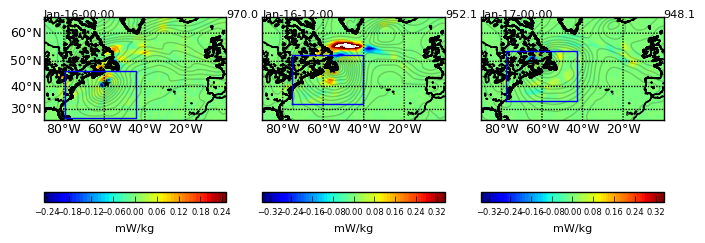
\includegraphics[width=36pc,angle=0]{Y:/Code_Data/Chapter2_3/Plots/Jan04_storm/ERA/plot_var_poly_ERA_diag500_msl_12UTC_15.png}
	\caption{Mean sea level pressure (contours) and diagnostic (filled contours) for ERA-Interim at 12 UTC 15th, 00 UTC 16th, 12 UTC 16th January 2004.The centre of this low pressure system is marked with a *. The time is on the top left of the plot and the minimum pressure on the top right (in hPa)}\label{fig:ERA_diag}
	\centering
\end{figure}

\begin{figure}	%%% remove [h] here and plots fell into place
	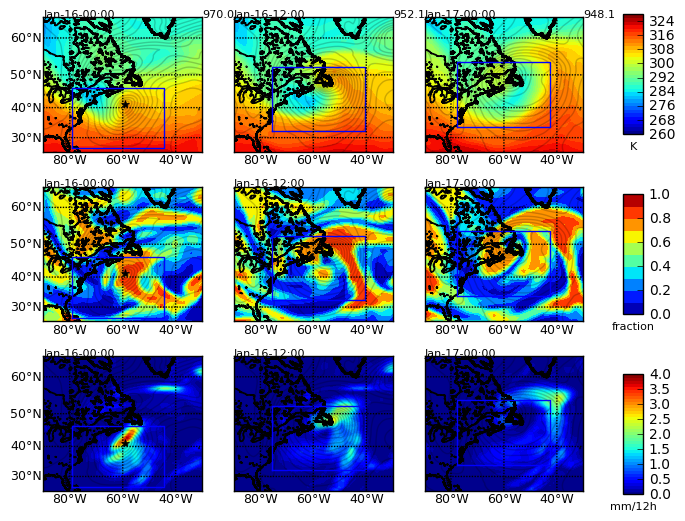
\includegraphics[width=36pc,angle=0]{Y:/Code_Data/Chapter2_3/Plots/Jan04_storm/ERA/plot_var_poly_ERA_ptRHprecip_12UTC_15.png}
	\caption{Filled contours: Top panels: 500 hPa potential temperature. Middle panels: 500 hPa relative humidity. Bottom panels: 12-hour precipitation centred on time. Mean sea level pressure is shown in contour line. ERA-Interim at 12 UTC 15th, 00 UTC 16th, 12 UTC 16th January 2004. The centre of this low pressure system is marked with a *. The time is on the top left of the plot and the minimum pressure on the top right (in hPa)}\label{fig:ERA_pt_RH_precip}
	\centering
\end{figure}

In 2004, the deterministic forecast member was at 0.5$^0$ degree resolution and so 3 grid points were used to create the low pass. Here (figure \ref{fig:fc_diag}), the shear diagnostic is larger than that in ERA-Interim, but smaller than that in the finer hindcast members. This storm has the lowest central pressure at each time step compared to ensemble member 9 and ERA-Interim, but this is likely to be due to the storm being approximately 12 hours ahead of the hindcast run. The precipitation in this single forecast member is more intense than that in ensemble member 9 and ERA-Interim.

\begin{figure}
	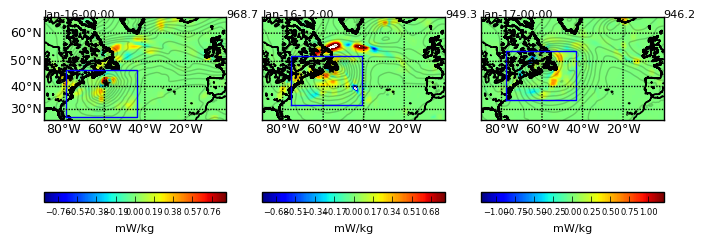
\includegraphics[width=34pc,angle=0]{Y:/Code_Data/Chapter2_3/Plots/Jan04_storm/FC_140104/plot_var_poly_fc_diag500_msl_12UTC_15.png}
	\caption{Mean sea level pressure (contours) and diagnostic (filled contours) for operational forecast at 12 UTC 15th, 00 UTC 16th, 12 UTC 16th January 2004.The centre of this low pressure system is marked with a *. The time is on the top left of the plot and the minimum pressure on the top right (in hPa)}\label{fig:fc_diag}
	\centering
\end{figure}

\begin{figure}	%%% remove [h] here and plots fell into place
	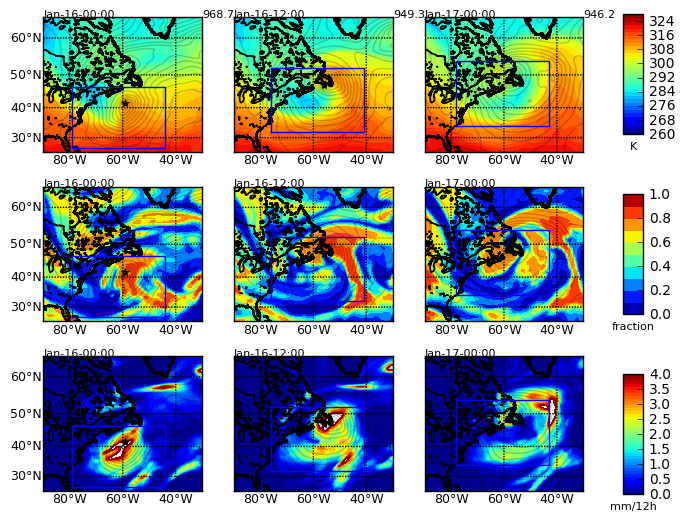
\includegraphics[width=36pc,angle=0]{Y:/Code_Data/Chapter2_3/Plots/Jan04_storm/FC_140104/plot_var_poly_fc_ptRHprecip_12UTC_15.png}
	\caption{Filled contours: Top panels: 500 hPa potential temperature. Middle panels: 500 hPa relative humidity. Bottom panels: 12-hour precipitation centred on time. Mean sea level pressure is shown in contour line. Operational forecast at 12 UTC 15th, 00 UTC 16th, 12 UTC 16th January 2004. The centre of this low pressure system is marked with a *. The time is on the top left of the plot and the minimum pressure on the top right (in hPa)}\label{fig:fc_pt_RH_precip}
	\centering
\end{figure}


These results suggest that with a high resolution model is required to resolve this shear instability. 

%PV from ERA and forecast
%Moist entrpoy


\subsection{Analysis in vertical cross-sections} \label{cx_analysis}

The following section shows vertical cross section analysis for ensemble member 9. The wind bars are calculated by taking the horizontal wind speed (m/s) and integrating this for an hour. The coloured contours show relative humdity and contour lines show potential temperature. The two line graphs show the shear diagnostic with height and horizontal distance (at 500 hPa), and precipitation is also shown in the horizontal plane. The original data did not include information on 600 hPa, so all values on this level are interpolated. The contours have data on 9 level (200, 300, 400, 500, 600, 700, 850, 925, 1000 hPa) and values in between are calculated by the plotting function.

% by multiplying by 3600 so give a horizontal distance each individual air parcel has moved. Metres into degrees by dividing by 110540. Plot the bar from start latitude to end latitude. Vertical movement, multiply omega (Pa/s) by 3600 and divide by 100 to get hPa/hour. Plot the line between the two start points and the two end points.

\begin{figure}[h]	
	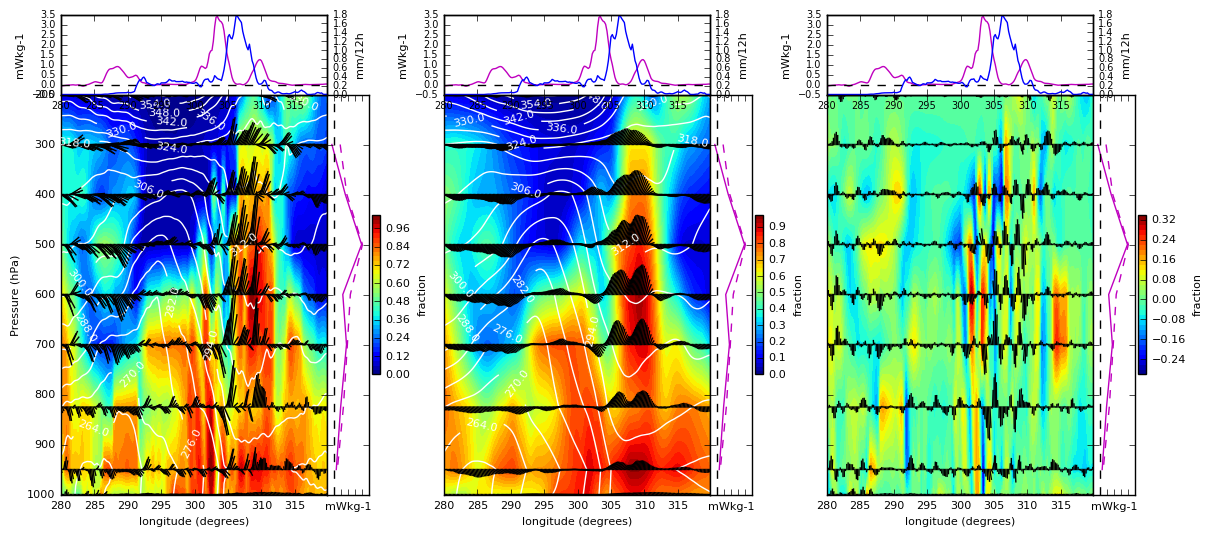
\includegraphics[width=40pc,angle=0]{Y:/Code_Data/Chapter2_3/Plots/Jan04_storm/HC_120104/cx3_sub_u_RH_pt_ens9_40N_12UTC_16th.png}
	\caption{Vertical cross-section on 12 UTC 16th at 40N. Relative humidity is shown in filled contours and isentropes are shown in white contour lines. Wind bars are calculated using zonal (u) and vertical ($\omega$) winds. The left hand plot shows the original data. The middle plot shows the low pass (wind bars, filled contours and contour lines), and the right hand plot shows the high pass (wind bars and filled contour lines). The horizontal line plots show the shear diagnostic in magenta and 12-hourly precipitation (mm) in blue. The vertical line plots show the mean diagnostic (solid magenta) and mean absolute diagnostic (dashed magenta).}\label{fig:HC_cxA}
	\centering
\end{figure}

At 12UTC 16th January (figure \ref{fig:HC_ens9}), the cold front is aligned north-south and a vertical cross-section at 40N is plotted to see the vertical motion and atmospheric characteristics across this front (figure \ref{fig:HC_cxA}). The wind bars show vertical motion throughout the depth of the troposphere, associated with a region of high relative humidity and high potential temperature. This ascent is in the warm, moist air in the warm sector of the cyclone, as the colder air behind the cold front undercuts this air mass and forces its ascent. The highest values of the shear instability diagnostic are seen in this region of high relative humidity and peak at 500 hPa. The precipitation peaks just to the west of this region, where there is a strong gradient in potential temperature. There is a second, smaller precipitation peak further west, just past the peak in the shear diagnostic.

%This descending air is also seen in the original and low pass wind bars.
%At 40N seems most intense. Also took sections at 38N and 42N and same pattern shown.
%Moist entropy only valid where saturated

%\begin{figure}[h]	
%	\includegraphics[width=40pc,angle=0]{Y:/Code_Data/Chapter2_3/Plots/Jan04_storm/HC_120104/cx3_sub_u_s_pt_ens9_40N_12UTC_16th.png}
%	\caption{Vertical cross-section 12 UTC 16th. s filled contours. pottemp and u 40N}\label{fig:HC_cxB}
%	\centering
%\end{figure}

%Cold front analysis - second time step, EW oriented - look at 38 or 39 N
%
%
\begin{figure}[h]	
	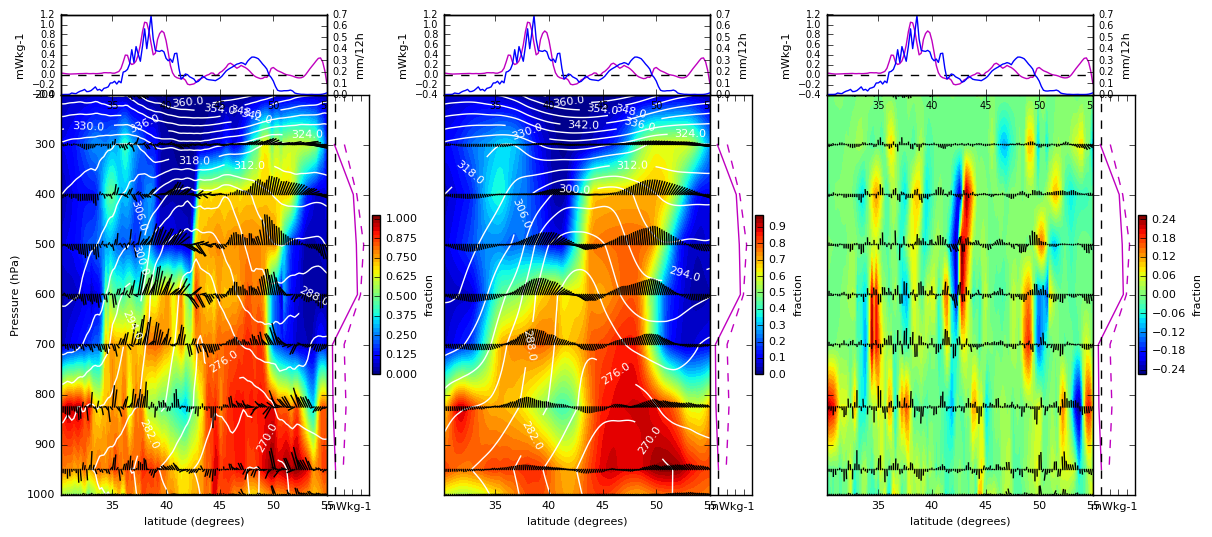
\includegraphics[width=40pc,angle=0]{Y:/Code_Data/Chapter2_3/Plots/Jan04_storm/HC_120104/cx3_sub_v_RH_pt_ens9_56W_00UTC_17th.png}
	\caption{Vertical cross-section on 00 UTC 17th at 56W. Relative humidity is shown in filled contours and isentropes are shown in white contour lines. Wind bars are calculated using meridional (v) and vertical ($\omega$) winds. The left hand plot shows the original data. The middle plot shows the low pass (wind bars, filled contours and contour lines), and the right hand plot shows the high pass (wind bars and filled contour lines). The horizontal line plots show the shear diagnostic in magenta and 12-hourly precipitation (mm) in blue. The vertical line plots show the mean diagnostic (solid magenta) and mean absolute diagnostic (dashed magenta).}\label{fig:HC_cxC}
	\centering
\end{figure}

Twelve hours later, at 00 UTC on 17th January, this cold front has changed position as the storm has evolved and is oriented east-west at around 36N to 40N. A section at 56W is taken and the v wind bars are plotted on a latitudinal plane (figure \ref{fig:HC_cxC}). The shear diagnostic is largest from 600 to 400 hPa, where there are large relative humidity values and ascent.


%\begin{figure}[h]	
%	\includegraphics[width=40pc,angle=0]{Y:/Code_Data/Chapter2_3/Plots/Jan04_storm/HC_120104/cx3_sub_v_s_pt_ens9_58W_00UTC_17th.png}
%	\caption{Vertical cross-section 00 UTC 17th. RH and v 58W}\label{fig:HC_cxC}
%	\centering
%\end{figure}

At 00 UTC on 17th and at approximately 52N, the warm front is aligned east-west if a section is taken at 45W. The warm front can be seen by the dip in the isentropes and this is in line with the peak in relative humidity and also two peaks in shear instability at 500 hPa.

\begin{figure}[h]	
	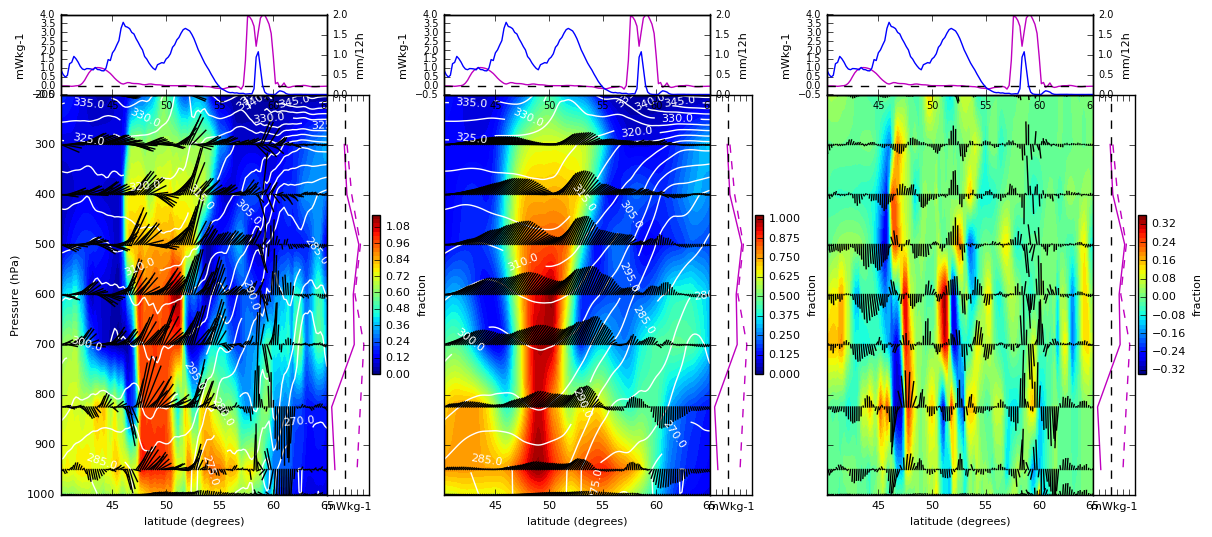
\includegraphics[width=40pc,angle=0]{Y:/Code_Data/Chapter2_3/Plots/Jan04_storm/HC_120104/cx3_sub_v_RH_pt_ens9_45W_00UTC_17th.png}
	\caption{Vertical cross-section on 00 UTC 17th at 45W. Relative humidity is shown in filled contours and isentropes are shown in white contour lines. Wind bars are calculated using meridional (v) and vertical ($\omega$) winds. The left hand plot shows the original data. The middle plot shows the low pass (wind bars, filled contours and contour lines), and the right hand plot shows the high pass (wind bars and filled contour lines). The horizontal line plots show the shear diagnostic in magenta and 12-hourly precipitation (mm) in blue. The vertical line plots show the mean diagnostic (solid magenta) and mean absolute diagnostic (dashed magenta).}\label{fig:HC_cxE}
	\centering
\end{figure}

%
%Through low pressure centre - capture some wf and some cf
%
%%\begin{figure}[h]	
%%	\includegraphics[width=40pc,angle=0]{Y:/Code_Data/Chapter2_3/Plots/Jan04_storm/HC_120104/cx3_sub_v_s_pt_ens9_52W_00UTC_17th.png}
%%	\caption{Vertical cross-section 00 UTC 17th. pottemp and v 57.4N}\label{fig:HC_cxF}
%%	\centering
%%\end{figure}
%
%\begin{figure}[h]	
%	\includegraphics[width=40pc,angle=0]{Y:/Code_Data/Chapter2_3/Plots/Jan04_storm/HC_120104/cx3_sub_v_RH_pt_ens9_52W_00UTC_17th.png}
%	\caption{Vertical cross-section 00 UTC 17th. pottemp and v 59N}\label{fig:HC_cxG}
%	\centering
%\end{figure}

%
%\subsection{Correlation analysis}
%
%%%%%%%%%%%%%%%%%%%%%%% SCATTER PLOTS %%%%%%%%%%%%%%%%%%%%%%%%%%%%
%Include all members and ERA and fc and MO amplitude of diagnostic. See a linear trend in terms of resolution and diagnostic strength?
%When do you reach the maximum strength? What is physically possible? asymptote?
%
%Talk about box following storm. Or just do over entire region, 1D correlation.
%%\begin{figure}
%	
%	\includegraphics[width=34pc,angle=0]{Y:/Code_Data/Chapter2_3/Plots/Jan04_storm/HC_120104/plot_var_poly_ctrl_diag500_msl_12UTC_15_3cb.png}
%	\caption{Mean sea level pressure (contours) and diagnostic (filled contours) for hindcast control at 12 UTC 15th, 00 UTC 16th, 12 UTC 16th January 2004.}\label{fig:HC_ctrl}
%	\centering
%\end{figure}

%Perhaps differences between ensembles because had previous storm that affected the path of this next storm

%Plots with SST contours?


These results have so far shown that shear instability can be resolved in all of the model simulations examined, although an increase in intensity is shown with an increase in resolution. This instability is strongly associated with the warm and cold fronts in the extra-tropical cyclone, with ascent seen throughout the depth of the troposphere. The instability peaks at around 500 hPa, which is consistent with other studies. Just one ensemble member from the 11-member hindcast has been presented here. However, large differences in storm characteristics can be seen between the different ensemble members.


\section {Future work}  

I hope to examine in more detail the relationship between the shear instability diagnostic and precipitation bands. I also aim to explore further the spread between the ensemble members. This work focussing on a single storm and the dynamics associated with this instability is important for setting up the work in the following chapter, where a climatology of storms will be analysed.



\section{Conclusions}
%Include limitations



